\documentclass[11pt,a4paper]{article}
\usepackage[margin=25mm]{geometry}
\usepackage{amsmath,amssymb,booktabs,graphicx,microtype}
\usepackage[hidelinks]{hyperref}
\usepackage[nameinlink,noabbrev]{cleveref}
\graphicspath{{../results/figures/}}

\title{Federated LPV Identification and Control\\\large Development Report}
\author{Jakob Weber}
\date{\today}

\begin{document}
\maketitle
\begin{abstract}
This living report develops and tests a federated LPV approach that separates
measurable operating-condition variation from persistent client heterogeneity.
The first stage is an oracle feasibility study. Only after the structural benefit
has been established will limited local data, learned clustering, uncertainty,
and communication constraints be introduced. The report will progressively
become the technical basis for a consolidated paper manuscript.
\end{abstract}
\tableofcontents

\section{Core idea}
The project separates two sources of variation that a frozen-model workflow can
confound:
\begin{equation}
  \text{measurable operating variation} \neq
  \text{persistent client heterogeneity}.
\end{equation}
For vehicle dynamics, longitudinal speed $\rho=v_x$ is measurable and varies
within a drive. Structural parameters such as mass, yaw inertia, and tire
cornering stiffness remain fixed for a client in the initial study. Client $i$ is
represented as
\begin{equation}
  x_{i,k+1}=A_i(\rho_k)x_{i,k}+B_i(\rho_k)u_{i,k},
\end{equation}
and is assumed to belong approximately to one persistent dynamics family $c(i)$:
\begin{equation}
  A_i(\rho)\approx A_{c(i)}(\rho),\qquad
  B_i(\rho)\approx B_{c(i)}(\rho).
\end{equation}
The central hypothesis is that LPV scheduling should explain operating-point
variation, whereas clustered federated learning should handle unknown persistent
structural variation. In geometric terms, the goal is to learn families of model
manifolds rather than clusters of unrelated frozen-model points.

\subsection{Research question and hypothesis}
\paragraph{Research question.}
Can federated system identification disentangle measurable operating-condition
variation from persistent fleet heterogeneity, enabling a heterogeneous fleet to
be represented and controlled by a small number of reusable LPV model and
controller families?

\paragraph{Hypothesis.}
Explicit LPV scheduling combined with structural specialization yields better
generalization and lower model/controller proliferation than either one global
LPV model or purely clustered LTI models.


\section{Motivation and practical value}
A frozen LTI model changes when the same vehicle is observed at different speeds.
Clustering those models without accounting for speed can therefore confuse an
operating point with a vehicle identity. An LPV description encodes that these
observations belong to one structural system evaluated at different values of a
known scheduling variable.

The distinction may reduce model and controller proliferation. A purely LTI
architecture can require approximately
\begin{equation}
  N_{\mathrm{families}}N_{\mathrm{speed\ regions}}
\end{equation}
calibrated controllers, whereas the proposed representation requires roughly one
scheduled controller family per relevant structural class. This matters for
calibration, deployment, validation, maintenance, and eventual certification.

Federation becomes particularly useful when individual clients cover only parts
of the scheduling range. Several compatible clients can jointly identify an LPV
family over an envelope that no single client has explored, without transferring
raw trajectories. Structural specialization simultaneously limits negative
transfer from physically incompatible clients. The full architecture separates
three questions:
\begin{center}
\begin{tabular}{lll}
\toprule
Quantity & Meaning & Mechanism\\
\midrule
$\rho(t)$ & current operating condition & LPV scheduling\\
$c_i$ & persistent dynamics family & clustering/personalization\\
$\Sigma_i$ & reliability of local evidence & uncertainty-aware federation\\
\bottomrule
\end{tabular}
\end{center}

This work continues the uncertainty-aware clustered identification and LQI design
pipeline developed for the IFAC study. Its new contribution is to give scheduling
variation and persistent fleet heterogeneity distinct mathematical roles.


\section{Related work and positioning}
\label{sec:related-work}

\subsection{LPV modeling and vehicle control}
LPV models represent dynamics whose coefficients depend on measurable scheduling
variables, providing a systematic alternative to independently designed frozen
controllers. Established LPV references cover identification, embedding choices,
gain scheduling, and stability analysis
\cite{toth2010lpv,apkarian1995selfscheduled,hoffmann2015survey}. Vehicle-control
studies have used LPV formulations to expose velocity dependence and tire
nonlinearities to scheduled controllers, including path-tracking designs validated
in high-fidelity simulation \cite{corno2021lpv,gimondi2021lpv}. The bicycle and
tire models used here follow the standard vehicle-dynamics hierarchy from linear
cornering stiffness to nonlinear saturation \cite{pacejka2012tire}.

This project does not claim novelty for representing vehicle dynamics as LPV or
for interpolating gains over speed. Its LPV contribution is representational:
known within-client operating variation is assigned to scheduling, so that
persistent between-client differences can be learned without proliferating
unrelated frozen-speed models.

\subsection{Federated learning under heterogeneity}
Federated averaging established the shared-model paradigm in which clients retain
their raw data and communicate locally computed updates \cite{mcmahan2017fedavg}.
When client objectives differ, federated multi-task and clustered methods replace
a single compromise model with structured sharing
\cite{smith2017federated,ghosh2020ifca,sattler2021clustered}. These methods motivate
family-specific aggregation, but generally treat heterogeneity as a statistical
or task-level property rather than separating a measured scheduling coordinate
from a persistent physical phenotype.

\subsection{Federated system identification and the research gap}
FedSysID studies collaborative identification when clients observe similar but
non-identical linear dynamical systems and quantifies the tradeoff between added
samples and system heterogeneity \cite{wang2023fedsysid}. This directly supports
the premise that a fleet can improve system identification through collaboration,
while also showing why unstructured global aggregation can become harmful as
physical differences increase.

The gap addressed here lies at the intersection of these bodies of work. Existing
LPV vehicle-control studies primarily assume a prescribed plant or centralized
identification; clustered FL methods learn multiple client models but do not
encode continuous operating-point variation; and current federated system
identification centers on shared or nearby fixed-system models. The proposed
architecture instead seeks a small number of \emph{LPV model manifolds}: each
family shares a speed-dependent model, while family membership captures persistent
vehicle heterogeneity. The oracle experiments in
\cref{sec:phase0,sec:phase1,sec:phase2,sec:phase3} first test whether this
decomposition is useful before any claim is made about recovering it from
decentralized data.

\section{Problem formulation}
Let the structural parameters of client $i$ be $\vartheta_i$ and the measured
scheduling variable be $\rho_k$. During the oracle study,
\begin{equation}
  \vartheta_i(t)=\vartheta_i,\qquad \rho_k=v_{x,k}\in[10,30]\,\mathrm{m\,s^{-1}}.
\end{equation}
The eventual hierarchical model is
\begin{equation}
 \Theta_i(\rho)=\Theta_{\mathrm{shared}}(\rho)
 +\Delta\Theta_{c(i)}(\rho)+\epsilon_i(\rho),
 \qquad \Theta=[A\ B].
\end{equation}
The first finite-dimensional LPV basis to test is
\begin{equation}
 \Theta(\rho)=\Theta_0+\rho^{-1}\Theta_1+\rho^{-2}\Theta_2.
\end{equation}
Phase~1 must validate this approximation before it is used for learning.

The controlled output is yaw rate $r$, with sideslip $\beta$ constrained through
the cost. A two-degree-of-freedom scheduled LQI architecture is considered:
\begin{equation}
 u=-K_x(\rho)x-K_I(\rho)\chi+k_r(\rho)r^\star.
\end{equation}
The same $Q$ and $R$ weights are used for all methods so that improvements cannot
be attributed to method-specific tuning.

\section{Vehicle benchmark}
\label{sec:benchmark}
The plant is the linear dynamic bicycle model with
$x=[\beta\ r]^\top$ and steering input $u=\delta$. Its parameters are
$\vartheta=[m,I_z,l_f,l_r,C_f,C_r]$. The initial centers are a nominal balanced
vehicle, a heavy/high-inertia vehicle, and a vehicle with a changed front--rear
handling balance. Ten clients per family receive modest fixed parameter scatter.
These values are initial hypotheses and will be checked for physical plausibility
and nontrivial but non-extreme separability during plant validation.
The relative centers used in the oracle study are listed in \cref{tab:families};
their absolute values and validated handling properties appear later in
\cref{tab:experiment0b-parameters}.

\begin{table}[ht]
\centering
\caption{Initial family centers relative to the nominal vehicle.}
\label{tab:families}
\begin{tabular}{lrrrr}
\toprule
Family & $m/m_0$ & $I_z/I_{z,0}$ & $C_f/C_{f,0}$ & $C_r/C_{r,0}$\\
\midrule
Nominal & 1.00 & 1.00 & 1.00 & 1.00\\
Heavy & 1.15 & 1.20 & 1.05 & 1.00\\
Handling balance & 0.95 & 0.90 & 0.90 & 1.10\\
\bottomrule
\end{tabular}
\end{table}

The training set combines independent lateral maneuvers and smooth speed profiles.
It also includes frozen-speed identification runs at
$12,16,20,24,28\,\mathrm{m\,s^{-1}}$. Test data contain unseen intermediate
speeds, unseen speed sequences, and a lateral maneuver with different timing and
amplitude. This separation is required to test dynamics generalization rather than
memorization of a speed--maneuver pairing.

\section{Experimental methodology}
\label{sec:methodology}
The study follows a gated progression:
\begin{equation}
\begin{split}
&\text{plant validation}\rightarrow\text{LPV representation validation}
\rightarrow\text{oracle model comparison}\\
&\rightarrow\text{oracle controller comparison}
\rightarrow\text{nonlinear-plant escalation}
\rightarrow\text{federated identification}.
\end{split}
\end{equation}
The early stages deliberately remove learning imperfections. This allows a
negative result to reject the structural premise before a federated algorithm is
developed. Results are first obtained for one deterministic development seed and
then repeated for ten independently sampled fleets and test-trajectory variants.

\subsection{Plant hierarchy}
The first plant is the speed-dependent linear bicycle model from
\cref{sec:benchmark}. It is LTI at a fixed speed but LPV across a drive:
\begin{equation}
 \dot x=A(v_x,\vartheta)x+B(v_x,\vartheta)\delta.
\end{equation}
It supports a clean test of the scheduling--specialization decomposition. After
this oracle test, the plant is replaced by a nonlinear bicycle model with
saturating hyperbolic-tangent tire forces. The identified models remain linear
LTI or LPV models. Thus, the second plant tests whether the compact abstraction
survives deliberate model mismatch.

\subsection{Compared model architectures}
\begin{table}[ht]
\centering
\caption{Core oracle model architectures.}
\label{tab:methods}
\begin{tabular}{llllr}
\toprule
Method & Scheduling & Specialization & Interpretation & Families\\
\midrule
M1: Global LTI & none & none & ignores both factors & 1\\
M2: Clustered LTI & none & oracle family & structure only & 3\\
M3: Global LPV & continuous & none & scheduling only & 1\\
M4: Clustered LPV & continuous & oracle family & both factors & 3\\
M5: Gridded LTI & discrete & family and speed & complex oracle & 15\\
\bottomrule
\end{tabular}
\end{table}
All methods receive equivalent data support. Controller comparisons use common
state and input weights. Method-specific tuning is prohibited unless it is
explicitly reported as a separate sensitivity analysis.

\subsection{Training and test separation}
Frozen-speed identification uses
$v_x\in\{12,16,20,24,28\}\,\mathrm{m\,s^{-1}}$. Interpolation tests include
$v_x\in\{14,18,22,26\}\,\mathrm{m\,s^{-1}}$. Varying-speed training trajectories
combine smooth speed profiles and lateral maneuvers independently so that speed
and maneuver identity are not confounded. Test data include unseen speeds, unseen
speed sequences, unseen lateral timing and amplitude, and unseen speed--maneuver
combinations.

\subsection{Common metrics}
Model metrics include one-step and free-run errors in sideslip and yaw rate, and
matrix errors
\begin{equation}
 E_A(v)=\lVert A_i(v)-\hat A(v)\rVert_F,\qquad
 E_B(v)=\lVert B_i(v)-\hat B(v)\rVert_F.
\end{equation}
Closed-loop metrics include yaw-rate tracking RMSE, sideslip RMS, steering RMS,
peak steering, peak steering rate, and the frozen-grid closed-loop spectral
radius. Every main result reports fleet mean, dispersion, worst-family result,
and family gap
\begin{equation}
 \Delta J_{\mathrm{family}}=\max_c J_c-\min_c J_c.
\end{equation}

\subsection{Experiment documentation contract}
Every experiment below is documented before execution using five fields:
objective, predeclared expectation, setup and evidence, decision gate, and
results/interpretation. The latter remains marked as pending until the experiment
has been run. Configuration, random seeds, output paths, and the producing Git
commit will be added with each result. Failed experiments and changed decisions
remain in this development report even if they are omitted from the final paper.


\section{Phase 0: plant and fleet validation}
\label{sec:phase0}
Phase~0 verifies the equations, discretization, operating envelope, and physical
family design before identification or control is introduced.

\subsection{Experiment 0A: nominal-vehicle validation}
\paragraph{Objective.}
Validate the nominal continuous and zero-order-hold-discretized bicycle model on
$v_x\in[10,30]\,\mathrm{m\,s^{-1}}$ with initial sample time
$T_s=0.01\,\mathrm{s}$.

\paragraph{Predeclared expectation.}
Matrix entries, poles, time constants, and steady-state gains vary smoothly with
speed. The nominal model is physically plausible and numerically well conditioned
over the complete envelope.

\paragraph{Setup and planned evidence.}
On a fine speed grid, compute continuous and discrete eigenvalues, controllability,
steady-state steering-to-yaw-rate and steering-to-sideslip gains, and an understeer
or equivalent handling measure. Plot selected $A$ and $B$ entries, pole
trajectories, and steady-state gains versus speed. Check equations, units, and sign
conventions independently.

\paragraph{Decision gate.}
No unintended instability, singularity, loss of controllability, discontinuity,
or implausible gain may occur. Any failure blocks all following experiments.

\paragraph{Results, interpretation, and decision.}
Pending.

\subsection{Experiment 0B: structural-family validation}
\paragraph{Objective.}
Verify that the nominal, heavy/high-inertia, and changed-handling-balance centers
create distinct but physically interpretable dynamics.

\paragraph{Predeclared expectation.}
The heavy family differs mainly in response speed and gain. The handling family
changes yaw/sideslip balance rather than merely rescaling the nominal response.

\paragraph{Setup and planned evidence.}
At $v_x\in\{12,20,28\}\,\mathrm{m\,s^{-1}}$, apply a small steering step, a smooth
sine sweep, and a lane-change-like input. Compare yaw rate, sideslip, poles,
steady-state gains, and family-to-family dynamic distance. Report a compact table
of absolute physical parameters and relative changes.

\paragraph{Decision gate.}
All centers must remain controllable and physically plausible. Differences must
be large enough to affect prediction and control, but not so extreme that the
benchmark makes family recovery trivial or unrealistic.

\paragraph{Results, interpretation, and decision.}
Pending.

\subsection{Experiment 0C: within-family client population}
\paragraph{Objective.}
Construct a 30-client fleet with ten clients per family and determine whether the
desired hierarchical structure is actually present.

\paragraph{Predeclared expectation.}
Client envelopes overlap modestly within each family. Persistent differences
between families remain visible over relevant parts of the speed range.

\paragraph{Setup and planned evidence.}
Sample bounded, fixed client parameters with initial ranges
$m,I_z:\pm2.5\%$ and $C_f,C_r:\pm5\%$. Inspect physical parameters, frozen-model
distances, response envelopes, and controllability over speed. The primary figure
shows family centers and within-family bands for selected dynamic characteristics.

\paragraph{Decision gate.}
Within-family variation should be smaller than between-family variation without
perfect separation on every scalar feature. Invalid samples are not silently
discarded; the sampling rule must be revised if they occur systematically.

\paragraph{Results, interpretation, and decision.}
Pending.

\subsection{Phase-0 benchmark freeze}
After Experiments 0A--0C pass, the equations, sample time, speed envelope, family
centers, scatter model, and development seed are frozen. Later changes require an
explicit report entry explaining the failure or new evidence that motivated them.

\section{Phase 1: LPV representation validation}
\label{sec:phase1}

\subsection{Experiment 1A: frozen-grid matrix approximation}
\paragraph{Objective.}
Select the smallest LPV basis that accurately represents the discretized bicycle
models between measured speed anchors.

\paragraph{Predeclared expectation.}
The physically motivated reciprocal-speed basis is likely effective, but exact
discretization may make a richer mixed basis necessary.

\paragraph{Setup and planned evidence.}
For every client, calculate exact frozen discrete matrices and fit
\begin{align}
 \Phi_1(v)&=[1,v],\\
 \Phi_2(v)&=[1,v^{-1},v^{-2}],\\
 \Phi_3(v)&=[1,v,v^{-1},v^{-2}].
\end{align}
Fit on the five training anchors and evaluate at unseen intermediate speeds and a
dense grid. Report absolute and normalized $E_A(v)$ and $E_B(v)$, worst-client
error, coefficient magnitude, and regression conditioning.

\paragraph{Decision gate.}
Choose the smallest basis with consistently low interpolation error and acceptable
conditioning. The originally proposed basis is rejected if the evidence favors a
different representation.

\paragraph{Results, interpretation, and decision.}
The comparison was run on all 30 clients for each of the ten robustness seeds,
giving 300 independently perturbed vehicles.  Each model was fit to exact ZOH
matrices at $v=\{12,16,20,24,28\}\,\mathrm{m\,s^{-1}}$.  The unseen points
$v=\{14,18,22,26\}\,\mathrm{m\,s^{-1}}$ measure interpolation, while a
201-point grid over $[10,30]\,\mathrm{m\,s^{-1}}$ also tests the two edge
intervals outside the fitting anchors.  Nonconstant feature columns were
standardized before least squares.  Table~\ref{tab:experiment-1a} reports the
combined relative error
\begin{equation}
 e_{AB}=\sqrt{\frac{1}{2}\left(e_A^2+e_B^2\right)},\qquad
 e_A=\frac{\lVert\widehat A_d-A_d\rVert_F}{\lVert A_d\rVert_F},
\end{equation}
with $e_B$ defined analogously.

\begin{table}[htbp]
 \centering
 \caption{Experiment 1A basis comparison over 300 clients.  Error entries are
 percentages; ``full worst'' includes edge extrapolation to 10 and
 $30\,\mathrm{m\,s^{-1}}$.}
 \label{tab:experiment-1a}
 \begin{tabular}{lrrrrr}
  \toprule
  Basis & Terms & $\kappa_2$ & Interp. mean & Interp. worst & Full worst \\
  \midrule
  $[1,v]$ & 2 & 1.00 & $3.222\!\times\!10^{-1}$ & $6.607\!\times\!10^{-1}$ & 2.255 \\
  $[1,v^{-1},v^{-2}]$ & 3 & 17.51 & $6.814\!\times\!10^{-5}$ & $2.711\!\times\!10^{-4}$ & $2.266\!\times\!10^{-3}$ \\
  Mixed & 4 & 140.72 & $1.820\!\times\!10^{-5}$ & $7.137\!\times\!10^{-5}$ & $1.065\!\times\!10^{-3}$ \\
  \bottomrule
 \end{tabular}
\end{table}

\begin{figure}[htbp]
 \centering
 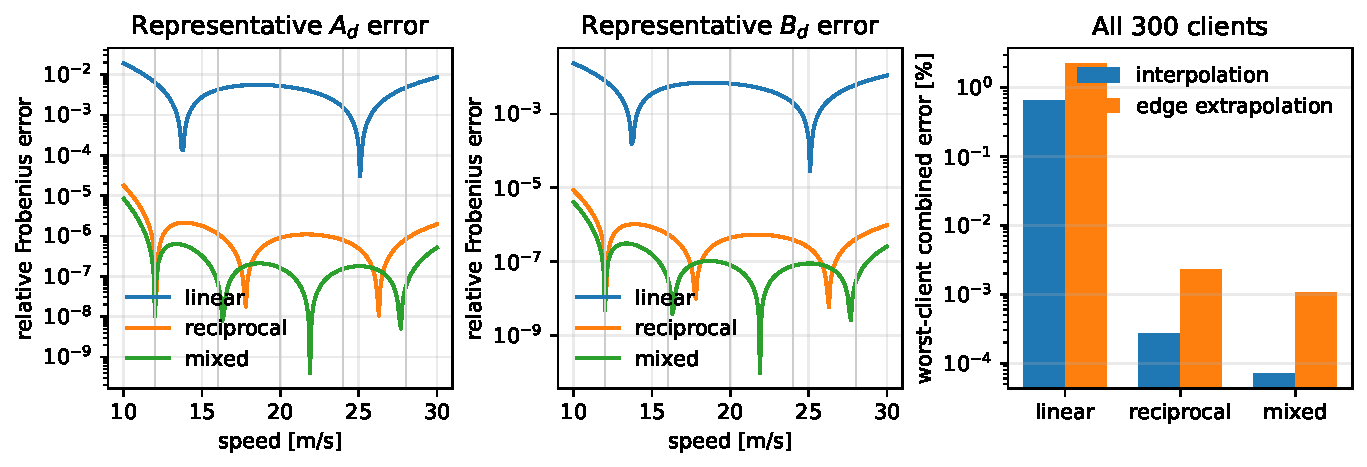
\includegraphics[width=\linewidth]{../results/figures/experiment_1a_basis_errors.pdf}
 \caption{Experiment 1A relative matrix errors.  The first two panels show a
 representative nominal client; gray lines mark fitting anchors.  The final
 panel gives population worst cases on a logarithmic scale.}
 \label{fig:experiment-1a}
\end{figure}

The error curves and population worst cases in \cref{fig:experiment-1a} confirm
the numerical ranking in \cref{tab:experiment-1a} over the full speed envelope.

The linear basis reaches a 2.26\% worst-case full-envelope error, which is too
large compared with the method differences that later experiments seek to
resolve.  The reciprocal basis reduces this error by roughly three orders of
magnitude to 0.00227\%.  Adding the $v$ term halves an already negligible error,
but increases the standardized design-matrix condition number from 17.5 to
140.7 and adds another coefficient matrix.  The largest reciprocal-basis error
occurs in edge extrapolation; its worst unseen-interpolation error is only
$2.71\times10^{-4}$\%.

Experiment 1A therefore passes.  We select and provisionally freeze
\begin{equation}
 \boxed{\Phi(v)=[1,v^{-1},v^{-2}]}
\end{equation}
as the smallest sufficiently accurate representation.  Experiment 1B must now
verify that this pointwise result remains accurate under time-varying simulation.

\subsection{Experiment 1B: varying-speed trajectory prediction}
\paragraph{Objective.}
Confirm that pointwise matrix accuracy translates into accurate speed-varying
simulation.

\paragraph{Predeclared expectation.}
The chosen LPV basis gives nearly exact one-step prediction and small, bounded
free-run error on the linear plant.

\paragraph{Setup and planned evidence.}
Use moderate persistently exciting steering with independent smooth profiles such
as $12\rightarrow20\rightarrow15$, $20\rightarrow28\rightarrow18$, and
$15\rightarrow25\rightarrow12\,\mathrm{m\,s^{-1}}$. Compare the true
speed-varying plant, exact frozen-matrix lookup, and fitted LPV model. Plot
representative states and error versus time, speed, and client family.

\paragraph{Decision gate.}
One-step errors must be negligible relative to the later between-method effects,
and free-run errors must not grow pathologically. Otherwise the basis or the
time-varying discretization treatment is revised before Phase~2.

\paragraph{Results, interpretation, and decision.}
The experiment used three smooth speed profiles,
$12\rightarrow20\rightarrow15$, $20\rightarrow28\rightarrow18$, and
$15\rightarrow25\rightarrow12\,\mathrm{m\,s^{-1}}$, each lasting 12 seconds.
All profiles were paired with the same independent three-frequency multisine
steering signal, whose peak magnitude is below $2.2^\circ$.  This common input
prevents speed and maneuver differences from being confounded.  The evaluation
again covered all 300 vehicles from the ten robustness seeds, for 900
trajectories in total.

The reference trajectory was integrated by fourth-order Runge--Kutta while
evaluating $A(v(t))$ and $B(v(t))$ continuously inside each sample.  Two
scheduled discrete models were propagated recursively: exact ZOH matrices
frozen at the left sample speed and the fitted reciprocal LPV matrices.  A third
comparison evaluates the LPV trajectory directly against the exact scheduled
discrete trajectory, thereby isolating basis approximation from the shared
sample-wise freezing error.  Relative errors are normalized by the RMS norm of
the corresponding reference state trajectory.

\begin{table}[htbp]
 \centering
 \caption{Experiment 1B one-step and free-run relative RMSE over 900
 trajectories. All error entries are percentages.}
 \label{tab:experiment-1b}
 \begin{tabular}{lrrrr}
  \toprule
  Comparison & 1-step avg. & 1-step max. & Free avg. & Free max. \\
  \midrule
  Exact frozen vs. continuous & $2.102\!\times\!10^{-3}$ & $3.275\!\times\!10^{-3}$ & $2.139\!\times\!10^{-2}$ & $3.339\!\times\!10^{-2}$ \\
  Reciprocal LPV vs. continuous & $2.116\!\times\!10^{-3}$ & $3.297\!\times\!10^{-3}$ & $2.184\!\times\!10^{-2}$ & $3.358\!\times\!10^{-2}$ \\
  Reciprocal LPV vs. exact frozen & $8.532\!\times\!10^{-5}$ & $1.725\!\times\!10^{-4}$ & $2.461\!\times\!10^{-3}$ & $6.112\!\times\!10^{-3}$ \\
  \bottomrule
 \end{tabular}
\end{table}

\begin{figure}[htbp]
 \centering
 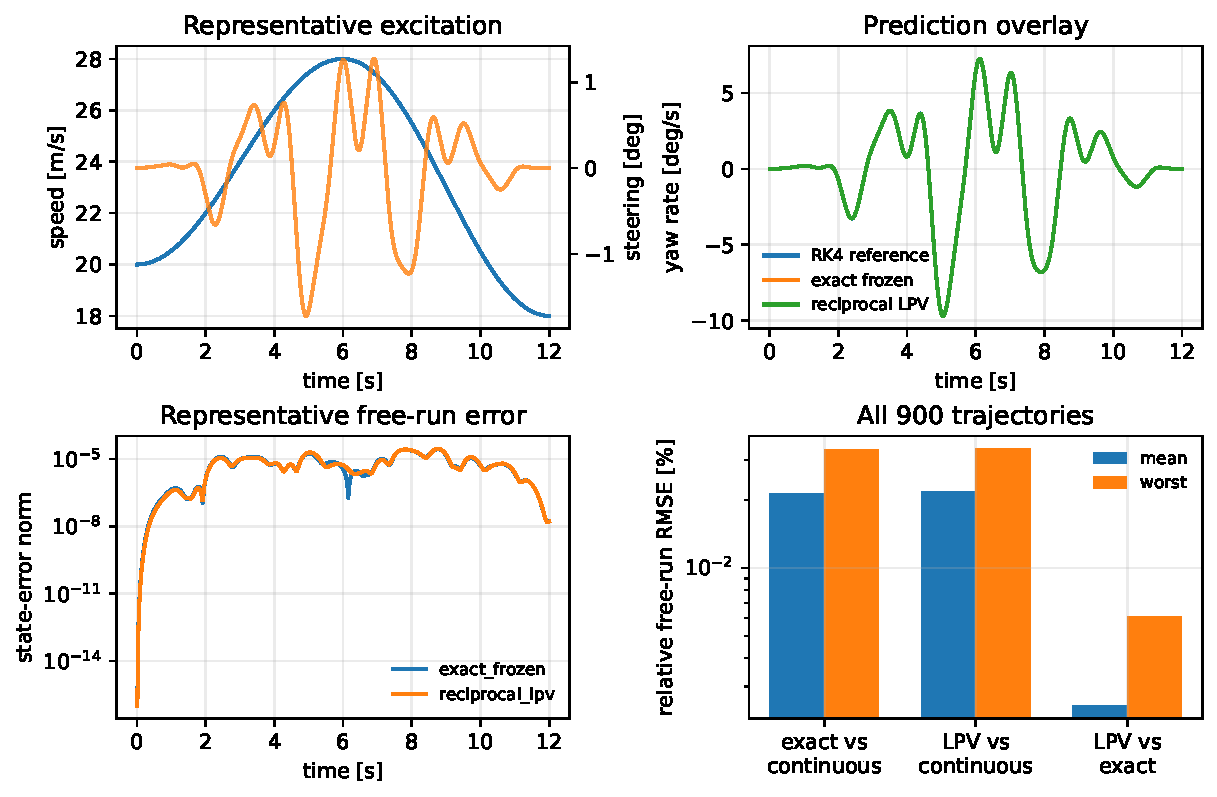
\includegraphics[width=0.92\linewidth]{../results/figures/experiment_1b_trajectory_validation.pdf}
 \caption{Experiment 1B varying-speed validation.  The scheduled predictions
 overlap visually with the continuous-time reference.  The lower panels expose
 the small free-run errors and distinguish the LPV basis error from the common
 within-sample speed-freezing error.}
 \label{fig:experiment-1b}
\end{figure}

The representative trajectories and separated error components are shown in
\cref{fig:experiment-1b}; the aggregate errors are reported in
\cref{tab:experiment-1b}.

The fitted LPV model is visually indistinguishable from both references.  Its
worst free-run error against the continuous-speed plant is only 0.0336\%, with
worst physical RMSEs of $4.78\times10^{-4}$ degrees in sideslip and
$1.15\times10^{-3}\,\mathrm{deg\,s^{-1}}$ in yaw rate.  Most of this discrepancy
is already present for exact frozen matrices.  The isolated reciprocal-basis
contribution has 0.00246\% mean and 0.00611\% worst free-run RMSE.  Its worst
one-step error is $1.73\times10^{-4}$\%.  Errors remain bounded throughout each
maneuver and decay with the faded input, rather than accumulating
pathologically.

Experiment 1B therefore passes.  The reciprocal representation is sufficiently
accurate that its approximation error is negligible relative to the effects
targeted in the oracle architecture comparison.

\subsection{Phase-1 representation freeze}
Experiments 1A and 1B jointly validate and freeze the Phase-1 representation:
\begin{itemize}
 \item scheduling basis $\Phi(v)=[1,v^{-1},v^{-2}]$;
 \item standardized nonconstant regression features;
 \item exact ZOH target matrices at $T_s=0.01\,\mathrm{s}$;
 \item fitting anchors $v=\{12,16,20,24,28\}\,\mathrm{m\,s^{-1}}$.
\end{itemize}
These choices remain fixed in the Phase-2 oracle comparison.  The validated
model is still the linear-tire bicycle plant; the nonlinear tanh-tire benchmark
remains a later robustness layer after the core architectural claim is tested.

\section{Phase 2: oracle model comparison}
\label{sec:phase2}
This is the first direct test of the central hypothesis. Family labels are known,
data are long and low-noise, and learning imperfections are intentionally absent.

\subsection{Experiment 2A: construct M1--M5}
\paragraph{Objective.}
Construct the architectures in \cref{tab:methods} under matched data support.

\paragraph{Setup and fairness rules.}
Global models pool all clients. Clustered models use true family labels. LTI
models are fitted across the same operating data as LPV models rather than at one
favorable speed. Aggregation is uniform initially. Uncertainty weighting and
learned clusters remain outside the oracle comparison.

\paragraph{Decision gate.}
All methods must pass numerical checks and use identical train/test splits. Model
errors are decomposed by method, speed, family, client, and trajectory.

\paragraph{Results, interpretation, and decision.}
Pending.

\subsection{Experiment 2B: isolate scheduling and specialization}
\paragraph{Objective.}
Determine whether scheduling and structural specialization solve distinct and
complementary errors.

\paragraph{Predeclared expectation.}
For speed variation within one family, LPV models outperform LTI models. At fixed
speed across families, specialized models outperform global models. With both
effects present, M4 outperforms M2 and M3.

\paragraph{Setup and planned evidence.}
Three diagnostic conditions are used:
\begin{enumerate}
 \item D1: one family over the full speed envelope;
 \item D2: all families at $v_x=20\,\mathrm{m\,s^{-1}}$;
 \item D3: all families under varying speed.
\end{enumerate}
Report one-step and free-run errors, error-versus-speed curves, worst-family error,
and family gap. After development, repeat with ten independently sampled fleets.

\paragraph{Decision gate.}
M4 must improve on both M2 and M3 in D3. A useful working gate is more than 10\%
for LPV relevance under broad speed variation and approximately 5--10\% for
specialization, with practical scale and seed consistency taking precedence over
the numerical thresholds. If M3 and M4 are equivalent, clustering is unnecessary.
If M2 and M4 are equivalent, LPV scheduling is unnecessary.

\paragraph{Results, interpretation, and decision.}
Pending.


\section{Phase 3: linear-plant controller oracle}
\label{sec:phase3}

\subsection{Experiment 3A: common controller architecture}
\paragraph{Objective.}
Translate model differences into a fair closed-loop comparison.

\paragraph{Setup.}
Augment the state with yaw-rate tracking error,
\begin{equation}
 \chi_{k+1}=\chi_k+T_s(r_k-r_k^\star),
\end{equation}
and use
\begin{equation}
 \delta_k=-K_x(v_k)x_k-K_I(v_k)\chi_k+k_r(v_k)r_k^\star.
\end{equation}
For LPV methods, calculate LQI gains at
$v\in\{10,15,20,25,30\}\,\mathrm{m\,s^{-1}}$ and interpolate them. Select common
$Q$ and $R$ once on the nominal vehicle and freeze them.

\paragraph{Planned evidence and decision gate.}
Audit controllability and closed-loop spectral radius for every client on a dense
speed grid. Gain interpolation must be continuous and all evaluated closed loops
must satisfy the predefined stability margin before simulation.

\paragraph{Results, interpretation, and decision.}
Pending.

\subsection{Experiment 3B: closed-loop scenarios C1--C4}
\paragraph{Objective.}
Test scheduling, specialization, their combination, and out-of-distribution
generalization in closed loop.

\paragraph{Predeclared expectation.}
LPV methods dominate for a fixed family under changing speed (C1), specialized
methods dominate across families at fixed speed (C2), M4 performs best when both
effects vary (C3), and its advantage survives unseen speed--maneuver combinations
(C4).

\paragraph{Setup and planned evidence.}
Use a smooth yaw-rate sine, single lane change, and double lane change/S-curve.
Measure yaw-rate RMSE, sideslip RMS, steering RMS, peak steering, peak steering
rate, worst-family result, and family gap. Plot one representative varying-speed
trajectory and aggregate distributions across clients and seeds.

\paragraph{Decision gate.}
M4 must improve tracking or family consistency without materially greater steering
effort. Benefits must survive C4. A method that wins only through aggressive input
or one favorable maneuver does not pass.

\paragraph{Results, interpretation, and decision.}
Pending.


\section{Phase 4: nonlinear-plant escalation}
\label{sec:phase4}
Phase~4 replaces the linear plant, not the compact identified model class. It tests
whether the structural conclusion survives realistic plant--model mismatch.

\subsection{Experiment 4A: nonlinear tire-model validation}
\paragraph{Objective.}
Implement and validate saturating tire forces
\begin{equation}
 F_{y,j}=C_j\alpha_{\mathrm{sat},j}
 \tanh\left(\frac{\alpha_j}{\alpha_{\mathrm{sat},j}}\right),
 \qquad j\in\{f,r\}.
\end{equation}

\paragraph{Predeclared expectation.}
The nonlinear plant agrees with the linear model at small slip and departs smoothly
as tire saturation becomes relevant.

\paragraph{Setup and planned evidence.}
Check the force--slip curves, small-signal slope, force limits, integration
accuracy, sideslip, yaw rate, and lateral acceleration. Preserve the Phase-0
structural families initially so that the plant change is isolated.

\paragraph{Decision gate.}
The model must have correct small-slip behavior, smooth saturation, plausible force
limits, and numerically converged simulations. Otherwise Phase~4 is blocked.

\paragraph{Results, interpretation, and decision.}
The nonlinear plant retains the Phase-0 state, input, structural family
parameters, and sign conventions. A common dry-road friction coefficient
$\mu=0.9$ is used. Static axle loads are
\begin{equation}
 F_{z,f}=mg\frac{l_r}{l_f+l_r},\qquad
 F_{z,r}=mg\frac{l_f}{l_f+l_r},
\end{equation}
and the saturation angles are selected as
\begin{equation}
 \alpha_{\mathrm{sat},j}=\frac{\mu F_{z,j}}{C_j}.
\end{equation}
Consequently, each tanh law has the original cornering stiffness at zero slip
and approaches the axle friction limit $\mu F_{z,j}$ smoothly. The resulting
family-center scales and force limits are listed in \cref{tab:experiment4a-tires}.

\begin{table}[htbp]
\centering
\caption{Experiment 4A tanh-tire parameters for the three Phase-0 family
centers at $\mu=0.9$.}
\label{tab:experiment4a-tires}
\begin{tabular}{lrrrr}
\toprule
Family & $\alpha_{\mathrm{sat},f}$ [deg] & $\alpha_{\mathrm{sat},r}$ [deg]
& $F_{y,f}^{\max}$ [kN] & $F_{y,r}^{\max}$ [kN]\\
\midrule
Nominal & 5.420 & 4.065 & 7.568 & 5.676\\
Heavy & 5.936 & 4.675 & 8.703 & 6.527\\
Handling & 5.721 & 3.511 & 7.189 & 5.392\\
\bottomrule
\end{tabular}
\end{table}

Central finite differences were used to linearize the nonlinear right-hand side
at zero sideslip, yaw rate, and steering for all family centers at
$v_x\in\{12,20,28\}\,\mathrm{m\,s^{-1}}$. The maximum relative Jacobian error
against the analytical Phase-0 matrices is $9.74\times10^{-13}$. Numerical force
curves are odd, monotone, have the prescribed zero-slip slope, and remain within
their friction limits.

Open-loop simulations use a smooth steering doublet at the same three speeds.
Three diagnostic amplitudes expose the transition from the linear limit to tire
saturation. Their worst results over all family--speed combinations are reported
in \cref{tab:experiment4a-responses}. These amplitudes validate the plant only;
Experiment 4B will independently select the final near-linear, moderate, and
strong-but-feasible maneuver levels.

\begin{table}[htbp]
\centering
\caption{Worst Experiment 4A nonlinear response diagnostics over the three
family centers and speeds $12$, $20$, and $28\,\mathrm{m\,s^{-1}}$. The model
difference is trajectory RMSE relative to the corresponding linear response.}
\label{tab:experiment4a-responses}
\begin{tabular}{lrrrr}
\toprule
Input & Amplitude [deg] & Model difference [\%] & Force utilization & $|a_y|_{\max}$ [$\mathrm{m\,s^{-2}}$]\\
\midrule
Small & 0.1 & 0.0084 & 0.032 & 0.274\\
Moderate & 2.0 & 3.705 & 0.595 & 5.121\\
Strong & 6.0 & 173.7 & 1.000 & 8.826\\
\bottomrule
\end{tabular}
\end{table}

The small input produces virtually identical linear and nonlinear trajectories.
The moderate input introduces a visible but controlled departure. The strongest
case drives at least one axle close to its friction limit and therefore separates
sharply from the unbounded linear-tire prediction, especially at high speed. All
27 nonlinear family--speed--amplitude simulations remain finite. These behaviors,
together with the tire curves, are summarized in
\cref{fig:experiment4a-validation}.

\begin{figure}[htbp]
 \centering
 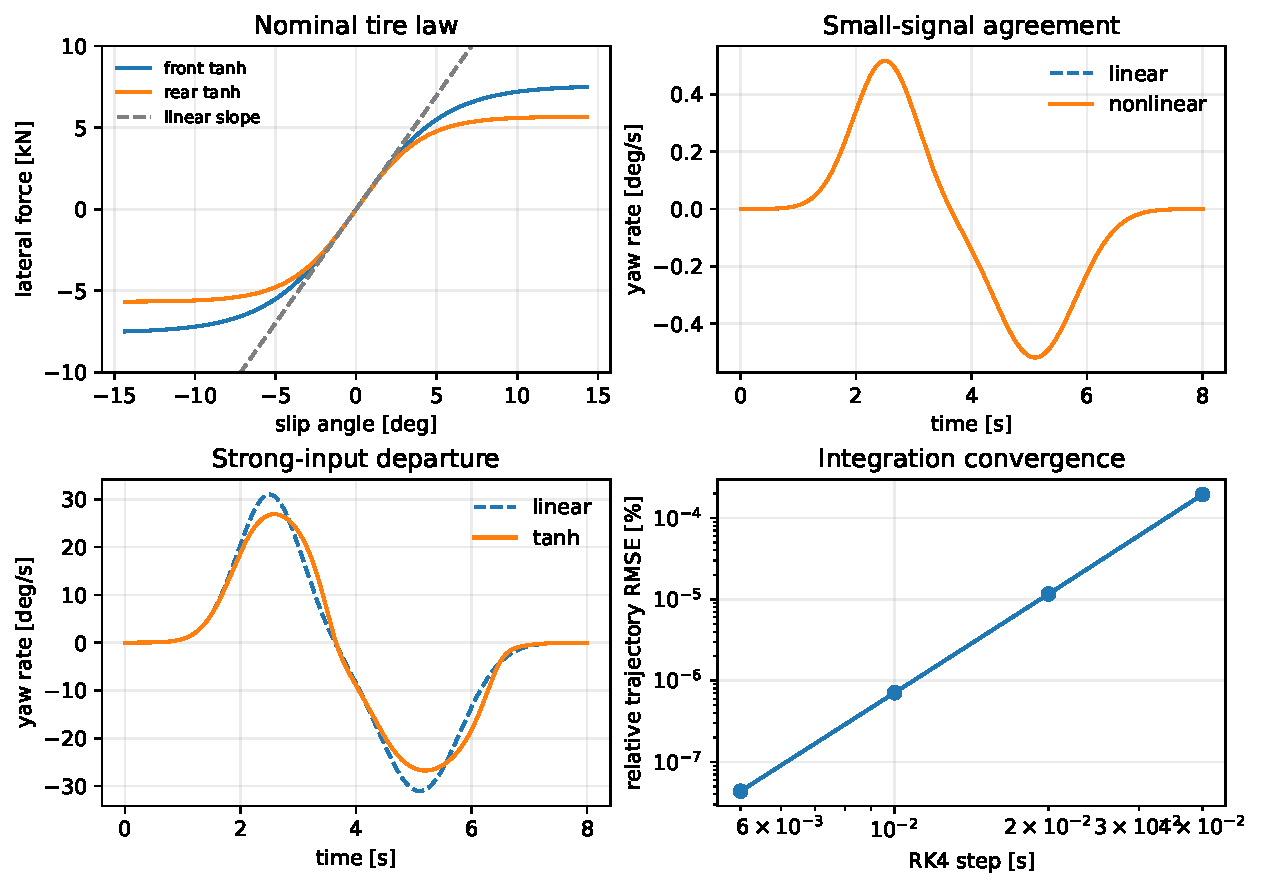
\includegraphics[width=0.95\linewidth]{experiment_4a_nonlinear_validation.pdf}
 \caption{Experiment 4A nonlinear-plant validation. The tanh tire law recovers
 the prescribed small-slip slope and saturates smoothly. The nonlinear vehicle
 matches the linear model under weak excitation and departs under strong
 excitation. The RK4 trajectory error decreases at the expected fourth-order
 rate.}
 \label{fig:experiment4a-validation}
\end{figure}

Integration was audited for the nominal $20\,\mathrm{m\,s^{-1}}$, $6^\circ$
case using RK4 steps from $40$ to $5\,\mathrm{ms}$ against a $1.25\,\mathrm{ms}$
reference. The relative trajectory error decreases by approximately a factor of
16 whenever the step is halved. At the retained $10\,\mathrm{ms}$ step it is
$7.10\times10^{-7}\%$, well below the predeclared $0.1\%$ gate.

Experiment 4A therefore \textbf{passes}. The nonlinear equations recover the
validated linear plant locally, provide bounded and physically interpretable tire
forces, and are numerically converged at the existing sample time. Experiment 4B
may proceed without changing the Phase-0 family definitions.
\subsection{Experiment 4B: maneuver-severity calibration}
\paragraph{Objective.}
Define reproducible near-linear, moderately nonlinear, and strongly nonlinear but
feasible operating levels.

\paragraph{Setup and planned evidence.}
Scale the lateral reference by
$\gamma_m\in\{0.5,1.0,1.5\}$. Report peak slip, lateral acceleration, tire-force
utilization, steering limits, and the fraction of time outside a predeclared
near-linear tire region. Adjust the absolute base maneuver once, globally, if the
three intended regimes are not obtained.

\paragraph{Decision gate.}
Severity levels must represent distinct regimes without making the strongest case
physically meaningless or infeasible for every linear controller.

\paragraph{Results, interpretation, and decision.}
Pending.

\subsection{Experiment 4C: oracle models under nonlinear mismatch}
\paragraph{Objective.}
Repeat M1--M5 using nonlinear-plant trajectories while retaining linear LTI/LPV
identified models.

\paragraph{Predeclared expectation.}
Absolute errors grow with maneuver severity, but the complementary benefits of
scheduling and specialization remain under moderate nonlinear excitation.

\paragraph{Setup and decision gate.}
Evaluate one-step and free-run error versus speed, family, and severity. The M4
advantage must survive at least the moderate regime and unseen speed--maneuver
combinations. If all linear LPV models fail, revise the representation before FL.

\paragraph{Results, interpretation, and decision.}
Pending.

\subsection{Experiment 4D: controller transfer and redesign}
\paragraph{Objective.}
Separate robustness of the Phase-3 controller from the achievable performance of
controllers redesigned using LPV approximations identified on nonlinear data.

\paragraph{Setup.}
The transfer test applies Phase-3 controllers unchanged. The redesign test refits
the compact models on nonlinear trajectories and synthesizes controllers with the
same common weights. The redesign test is primary; transfer is diagnostic.

\paragraph{Decision gate.}
The qualitative M4 benefit should survive moderate excitation. If it survives only
near the linear region, the claim and operating envelope are restricted
explicitly. Frozen-grid checks are necessary but are not presented as a formal LPV
stability certificate.

\paragraph{Results, interpretation, and decision.}
Pending.

\subsection{Experiment 4E: control-relevant identification diagnosis}
\label{sec:experiment4e}
\paragraph{Question and controlled comparisons.}
Does redesign fail because of numerical solution error, nonlinear training
amplitudes, or limitations already present in pooled linear-plant identification?
The same seed-1 fleet, collection controller, two training profiles, and held-out
moderate S-curve are retained. Compare original nonlinear-data regression,
column-scaled SVD solving the same ridge objective, SVD using only near-linear
nonlinear trajectories, and SVD using linear-plant trajectories at all three
amplitudes. The last case uses exact frozen-speed ZOH propagation for training.
All redesigned controllers are tested on the nonlinear plant.

For regression matrix $X$, define $S_{jj}=\|X_{:j}\|_2$. The numerical check is
\begin{equation}
 \min_W\left\|\begin{bmatrix}XS^{-1}\\\sqrt{\epsilon}S^{-1}\end{bmatrix}W
 -\begin{bmatrix}Y\\0\end{bmatrix}\right\|_F^2,
 \qquad \widehat\Theta^{\mathsf T}=S^{-1}W,\quad\epsilon=10^{-10}.
\end{equation}
Scaling changes the solver, not the regularization objective. M1, M2, and M5
retain their original solver. A small absolute ridge coefficient is not
necessarily negligible relative to weak regressor directions.

\paragraph{Results.}
\Cref{tab:experiment4e} shows that SVD reproduces the original M4 failure.
Pooled raw condition numbers are approximately $1.46$--$1.80\times10^6$,
falling to $5.86$--$7.76\times10^3$ after column scaling. All matrices have
full column rank, but weak directions remain. The solver change alters M4
tracking by less than $10^{-9}\,\mathrm{deg\,s^{-1}}$. Numerical roundoff
therefore does not explain the observed failure.

\begin{table}[htbp]
\centering
\caption{Experiment 4E: M4 diagnosis. Tracking is moderate-test yaw RMSE in
$\mathrm{deg\,s^{-1}}$. Relative $B$ error is averaged over clients and 161
speeds against each client's true small-signal matrix.}
\label{tab:experiment4e}
\begin{tabular}{lrrr}
\toprule
Identification data and solver & Tracking & Worst $\rho$ & Relative $B$ error\\
\midrule
Nonlinear, all amplitudes, original & 0.05737 & 1.0321 & 0.4633\\
Nonlinear, all amplitudes, SVD & 0.05737 & 1.0321 & 0.4633\\
Nonlinear, near-linear only, SVD & 0.06255 & 0.9770 & 0.4715\\
Linear plant, all amplitudes, SVD & 0.06147 & 0.9772 & 0.4679\\
\bottomrule
\end{tabular}
\end{table}

The original worst M4 instability occurs at $12\,\mathrm{m\,s^{-1}}$ for
handling\_07. Near-linear training restores frozen M4 stability, but does not
improve tracking. Linear-plant training also leaves substantial input-matrix
error and poor tracking. Global LPV remains unstable in both ablations.
Nonlinear tire mismatch is therefore not the sole explanation. Relative matrix
errors use the fixed state coordinates and are not coordinate-invariant metrics.

\Cref{fig:experiment4e} relates input-channel error, gain, and stability for a
representative heavy client. Complete client and speed results accompany the
report as CSV files. Inspection confirms the same $r-r^\star$ integrator
convention, radian states and inputs, and prefilter equilibrium equation in
synthesis and simulation. Existing controller tests pass, providing no evidence
of a sign or unit error without claiming exhaustive software verification.

\begin{figure}[htbp]
\centering
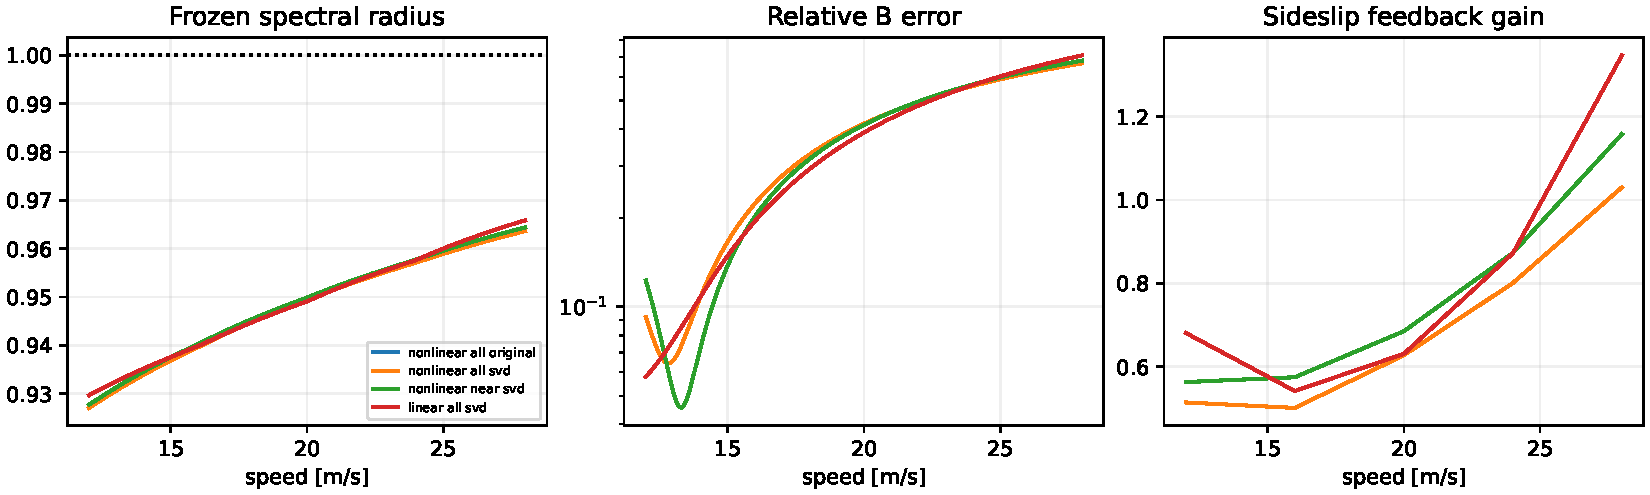
\includegraphics[width=\linewidth]{experiment_4e_diagnosis.pdf}
\caption{Experiment 4E for heavy\_00. Original and SVD all-amplitude curves
overlap. This representative client is not the fleet's worst-case client.}
\label{fig:experiment4e}
\end{figure}

\paragraph{Interpretation and decision.}
Training uses two fixed speed--maneuver pairings, not their full cross product.
Pooled clients have different dynamics even within a family, and the reciprocal
basis only approximates exact discrete-time dynamics. Weak excitation, pooling
mismatch, basis approximation, and ridge bias can interact. Their individual
causal contributions have not all been isolated. The demonstrated finding is
that a solver change or reduced tire excitation alone does not recover the
desired performance. Experiment 4F reduces the degrees of freedom through
physical relationships while keeping controller weights fixed.

A further linear-data check fits nominal\_00, heavy\_00, and handling\_00
separately using their own trajectories. Mean relative $B$ errors are
$2.29$--$4.20\times10^{-5}$ without ridge and
$2.68$--$3.83\times10^{-4}$ with the original ridge. These are far below
the pooled M4 error of $0.468$. This strongly implicates heterogeneous pooling
under the existing closed-loop data distribution, rather than an inability of
the basis to represent each individual client. It does not isolate pooling from
all interactions with excitation. In closed loop, regression coefficients can
compensate along correlated state--input directions, so the pooled best predictor
need not equal an average of the individually identified physical models.

\subsection{Experiment 4F: structured local-dynamics identification}
\label{sec:experiment4f}
\paragraph{Method and information boundary.}
Fit near-linear nonlinear-plant trajectories using three positive ratios
\begin{equation}
 p=(a_f,a_r,h)=\left(C_f/m,\ C_r/m,\ m/I_z\right).
\end{equation}
Only the common geometry $l_f=1.2\,\mathrm m$, $l_r=1.6\,\mathrm m$ is known
to the estimator. True client mass, inertia, and stiffnesses are not supplied.
The continuous matrices satisfy
\begin{equation}
 A_c(v;p)=\begin{bmatrix}
 -(a_f+a_r)/v & (a_rl_r-a_fl_f)/v^2-1\\
 h(a_rl_r-a_fl_f) & -h(a_fl_f^2+a_rl_r^2)/v
 \end{bmatrix},\qquad
 B_c(v;p)=\begin{bmatrix}a_f/v\\ha_fl_f\end{bmatrix}.
\end{equation}
This avoids attempting to recover individually unidentifiable absolute physical
quantities. The estimator minimizes one-step RK4 residuals at $0.01$ s, scaled
by $0.05^\circ$ and $0.5^\circ\mathrm{/s}$ for sideslip and yaw rate.
Logarithmic parameters enforce positivity, with bounds $a_f,a_r\in[1,300]$
and $h\in[0.05,3]$ in corresponding SI units. Two common starting points,
$(40,40,0.5)$ and $(80,60,1)$, are used for each group. Training loss selects
the solution, with no held-out tracking-based selection. These are effective
group fits, not claimed exact family-center recovery.

\paragraph{Architecture comparison and changed estimation procedure.}
One structured fit is obtained globally and one per oracle family. M3 and M4
evaluate them continuously in speed. M1 and M2 freeze the corresponding fit at
the preselected $20\,\mathrm{m\,s^{-1}}$. M5 uses five frozen family fits
with nearest-anchor switching. All architectures receive the same structural
prior. This differs from 4D's independently optimized constant and gridded
regressions: 4F isolates deployment architecture after common identification.
It does not establish dominance over every LTI fitting procedure. Earlier
4D and 4E baselines remain part of the record.

Synthesis uses exact frozen-speed ZOH matrices, unchanged $Q,R$, and the existing
gain grid. Tests verify the reduced matrices against the validated physics and
RK4 against ZOH. Scaled local residual-Jacobian condition numbers are
$1.33$--$1.87$. Both starts agree within $9\times10^{-8}$ relative difference.
These support local numerical identifiability, not a global proof.

\paragraph{Results and gate.}
\Cref{tab:experiment4f} gives the moderate results. M4 reduces mean tracking
error by $8.7\%$ relative to structured M2 and $9.1\%$ relative to structured
M3. It approaches the physics-transfer value $0.03464$ without blending with
oracle matrices. Near-linear and strong M4 tracking errors are $0.01644$ and
$0.05678\,\mathrm{deg\,s^{-1}}$. All architectures are amplitude-feasible
at all three severities.

\begin{table}[htbp]
\centering
\caption{Experiment 4F: structured identification and redesign. Tracking and
worst-family values are yaw RMSE in $\mathrm{deg\,s^{-1}}$.}
\label{tab:experiment4f}
\begin{tabular}{lrrr}
\toprule
Architecture & Mean tracking & Worst family & Worst frozen $\rho$\\
\midrule
M1 & 0.04065 & 0.04340 & 0.9619\\
M2 & 0.03775 & 0.03831 & 0.9646\\
M3 & 0.03792 & 0.04453 & 0.9643\\
M4 & \textbf{0.03446} & \textbf{0.03636} & 0.9663\\
M5 & 0.04228 & 0.04270 & 0.9663\\
\bottomrule
\end{tabular}
\end{table}

The initial recovery gate passes: M4 is feasible, passes the frozen-grid audit,
and improves tracking by over $5\%$ against both structured alternatives.
This is one fleet with unseen trajectories on the same clients. Frozen
stability is not a time-varying LPV certificate. Next, validate independent
fleet seeds and additional speed--maneuver combinations, including the original
fitted LTI baselines. Only then introduce local identification, federation, and
learned clustering. Structured local-dynamics identification is a promising
repair, not evidence of universal M4 superiority.

\subsection{Experiment 4G: independent-fleet and trajectory validation}
\label{sec:experiment4g}
\paragraph{Purpose and frozen protocol.}
Experiment 4F recovered the expected architecture advantage on one fleet, but
used the same clients for identification and testing. Experiment 4G tests whether
that recovery transfers to independently sampled vehicles and additional
trajectories. Training seeds are 11--20, paired with test seeds 111--120. Each
fleet contains ten clients in each of the three unchanged physical families.
Thus 300 training and 300 separate test vehicles are used. Test clients share
the family distribution, not the realized physical parameters, with training
clients. Repeated textual client IDs are scoped by fleet seed.

All estimator bounds, starts, residual scaling, geometry assumptions, controller
weights, and speed grids remain those of 4F. The physics controller used for
data collection is constructed from the training fleet only. Structured fitting
uses near-linear training records only. No test trajectories or test-plant
matrices enter identification, tuning, or candidate selection. True test plants
are accessed only for simulation and the post-design frozen audit. Family labels
remain oracle information. The JSON protocol is frozen before the runs and its
SHA-256 digest is stored with the conclusions.

\paragraph{Comparators and additional trajectories.}
The five structured architectures retain the definitions in
\cref{sec:experiment4f}. Two additional clustered LTI baselines fit constant
matrices directly: LTI-all uses all three training amplitudes, reproducing 4D's
estimation approach, while LTI-near uses precisely the same near-linear records
as structured M4. A training-physics M4 transfer controller supplies a reference.
This separates the structured-LTI baseline choice from a claim against the
original directly fitted LTI controllers.

Each frozen controller is evaluated on three 12 s scenarios:
\begin{enumerate}
\item the previous held-out S-curve with $28\rightarrow16\rightarrow24$ m/s;
\item a shifted double lane change with $16\rightarrow27\rightarrow19$ m/s,
using opposite Gaussian yaw pulses of amplitude $8.5^\circ$/s, centered at
3.8 and 7.4 s with widths 0.85 and 0.65 s;
\item an unseen constant speed of 22 m/s and an enveloped sinusoidal yaw
reference, in degrees/s,
\[
 r^\star(t)=7.5\sin^2(\pi t/12)\sin(2\pi\,0.18t+0.35).
\]
\end{enumerate}
Every reference is scaled by 0.5, 1, and 1.5. The labels near-linear, moderate,
and strong denote these inherited amplitude factors. The additional maneuvers
have not been recalibrated to equal tire-force utilization. Speed remains in
the identification support. These tests concern interpolation and new maneuver
combinations, not extrapolation to new physical families or speeds.

\paragraph{Statistical unit and decision rule.}
Moderate-severity tracking is primary. For each train/test seed pair, average
equally over the three scenarios and the balanced test fleet. Paired differences
are baseline RMSE minus M4 RMSE. Confidence intervals resample the ten seed pairs
10,000 times with bootstrap seed 4107, preserving all within-fleet dependencies.
They are pointwise 95\% bootstrap intervals, not simultaneous significance
statements. Individual clients and scenarios are not treated as independent
replicates. Per-scenario contrasts and near-linear/strong outcomes are secondary.

The recovery gate requires at least 5\% reduction in the ratio of mean primary
RMSEs and a positive lower confidence bound against structured M2, structured
M3, LTI-all, and LTI-near. M4 must also be amplitude-feasible in every run and
have spectral radius below one on every held-out frozen audit point. The audit
uses 161 speeds in $[12,28]$ m/s and is not a time-varying LPV certificate.
No failed client or seed is excluded. A vectorized simulator accelerates fleet
evaluation and is tested against the original scalar RK4 simulator and metrics.

\paragraph{Results and interpretation.}
All ten seed pairs completed, yielding 21,600 closed-loop evaluations across
eight methods, three scenarios, three amplitude factors, and 300 held-out
clients. \Cref{tab:experiment4g-means} reports the primary fleet averages and
variation across seed pairs. Structured M4 nearly matches the training-physics
controller, while outperforming both structured alternatives and the original
directly fitted LTI baselines. Its average worst-family error is also smaller
than those of the learned comparators.

\begin{table}[htbp]
\centering
\caption{Experiment 4G: moderate tracking, averaged equally over three scenarios.
Mean, seed standard deviation, and mean worst-family RMSE are in degrees/s.
Worst-family values take the maximum family mean within each seed pair before
averaging across pairs.}
\label{tab:experiment4g-means}
\begin{tabular}{lrrr}
\toprule
Method & Mean $\pm$ seed SD & Worst family & Worst frozen $\rho$\\
\midrule
Structured M1 & $0.03723\pm0.00067$ & 0.04487 & 0.9625\\
Structured M2 & $0.03341\pm0.00066$ & 0.03430 & 0.9653\\
Structured M3 & $0.03222\pm0.00063$ & 0.03766 & 0.9648\\
Structured M4 & $\mathbf{0.02757}\pm0.00041$ & 0.02842 & 0.9668\\
Structured M5 & $0.03342\pm0.00057$ & 0.03455 & 0.9668\\
Direct LTI-all & $0.03528\pm0.00242$ & 0.05430 & 0.9639\\
Direct LTI-near & $0.03314\pm0.00224$ & 0.05044 & 0.9625\\
Physics M4 reference & $0.02752\pm0.00043$ & 0.02830 & 0.9668\\
\bottomrule
\end{tabular}
\end{table}

\Cref{tab:experiment4g-paired} gives the paired evidence. All four primary
contrasts favor M4 in all ten seed pairs, with strictly positive interval lower
bounds and reductions exceeding 5\%. Thus the frozen recovery gate passes.
The direct-LTI comparisons are especially relevant: the improvement is not
confined to the frozen structured LTI baseline introduced in 4F.

\begin{table}[htbp]
\centering
\caption{Experiment 4G paired moderate tracking contrasts. $\Delta$ is baseline
minus M4 RMSE in degrees/s. Intervals bootstrap the ten complete seed pairs.}
\label{tab:experiment4g-paired}
\begin{tabular}{lrrr}
\toprule
Baseline & M4 reduction & Mean $\Delta$ & 95\% interval for $\Delta$\\
\midrule
Structured M2 & 17.5\% & 0.00584 & $[0.00565,0.00602]$\\
Structured M3 & 14.4\% & 0.00465 & $[0.00433,0.00497]$\\
Direct LTI-all & 21.9\% & 0.00771 & $[0.00637,0.00901]$\\
Direct LTI-near & 16.8\% & 0.00558 & $[0.00433,0.00677]$\\
\bottomrule
\end{tabular}
\end{table}

\Cref{fig:experiment4g} shows that the aggregate result is supported by each
scenario. Against structured M2, M4 improves by 9.1\% on the original S-curve,
31.1\% on the shifted lane change, and 9.8\% at constant 22 m/s. Against
direct LTI-near, the reductions are 11.3\%, 28.4\%, and 8.5\%. The last
comparison favors M4 in nine of ten individual pairs, so scenario-wise
dominance is not universal. Constant-speed performance reflects selecting an
appropriate scheduled gain away from the LTI design speed, not time variation
within that particular run. M5 chooses its lower nearest anchor at the 22 m/s
tie, which explains its equality with structured M2 in this scenario.

\begin{figure}[htbp]
\centering
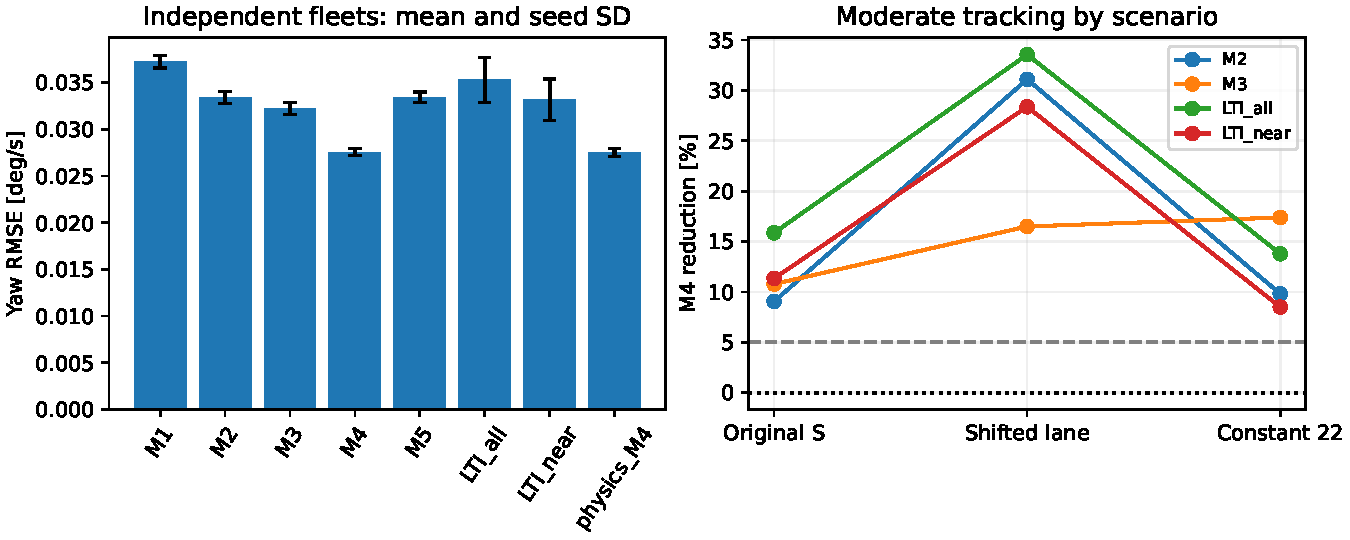
\includegraphics[width=\linewidth]{experiment_4g_validation.pdf}
\caption{Experiment 4G. Left: moderate tracking averaged over scenarios, with
seed standard deviations. Right: relative M4 benefits by scenario. Dashed gray
marks the 5\% aggregate practical threshold, not a separate scenario gate.}
\label{fig:experiment4g}
\end{figure}

All methods remain amplitude-feasible in every evaluated trajectory. Structured
M4 has worst held-out frozen spectral radius 0.9668. Its near-linear and strong
mean RMSEs are $0.01321\pm0.00020$ and $0.04532\pm0.00068$ degrees/s. The
physics reference is approximately 0.17\% better on the aggregate moderate
metric. Consequently, the result supports recovery of useful physics-controller
performance from data, not superiority to known physics. Absolute differences
are small and must be considered alongside their relative percentages.

\paragraph{Scope and next decision.}
The independent-fleet recovery is supported within the original family
distribution, known geometry, noise-free state measurements, two training
profile pairings, and three deterministic test scenarios. It does not establish
robustness to new family centers, sensor noise, limited speed coverage, learned
family assignments, or arbitrary scheduling rates. No formal time-varying
stability certificate is claimed. The structured identification route now has
stronger oracle support than 4F alone. The subsequent complexity and regime
studies can use this validated route, while finite local information and
federated recovery remain distinct questions. No federated learning claim follows
from this centralized oracle experiment.

\section{Phase 5: model and controller complexity}
\label{sec:phase5}

\subsection{Experiment 5A: LTI-prototype sweep}
\label{sec:experiment5a}
\paragraph{Objective and refinement of the original plan.}
After the independent-fleet validation in \cref{sec:experiment4g}, determine
how many frozen gains approximate M4's three scheduled families. The original
generic cluster-count sweep is refined to $n\in\{1,2,3,5,8,10\}$ speed anchors
per known family, hence $3n$ frozen controllers. This isolates speed
discretization while keeping structural specialization and identification fixed.
It is not a learned-clustering study.

\paragraph{Frozen setup and selection boundary.}
Reuse the ten 4G training/test seed pairs and their stored structured parameter
fits. Both M4 and LTI grids use these same fits and unchanged $Q,R$. For $n>1$,
candidate layouts are equally spaced endpoint-inclusive anchors over $[12,28]$
m/s, equal-cell centers, and training-speed quantiles at probabilities
$(j+1/2)/n$, $j=0,\ldots,n-1$. For $n=1$, compare 16, 20, and 24 m/s.
Each grid is shared across the three families. For every count, select the
amplitude-feasible candidate with smallest mean yaw RMSE on the two original
moderate training maneuvers and the training fleet. This is a finite
training-based search, not an optimal placement claim. No test metric enters
anchor selection.

Selected LTI grids use nearest-anchor switching, with the lower anchor at ties.
M4 retains interpolation over its five fixed anchors. Test the same three
scenarios and three amplitude factors as 4G on independent test clients.
Report tracking, steering RMS, peak steering rate, switch counts, amplitude
feasibility, and frozen stability. Neither method receives hysteresis,
smoothing, steering-rate limiting, or feedback-weight retuning.

\paragraph{What is counted.}
All methods originate from three fits with three parameter ratios each. Thus
this study cannot claim fewer independently learned models for M4. M4 deploys
15 gain vectors, each with three feedback coefficients and one prefilter,
plus five shared speed anchors: 65 scalars. A frozen grid deploys $3n$ vectors
and $n$ shared anchors: $13n$ scalars. Counts exclude common software, units,
labels, and metadata. Retaining explicit frozen $A,B$ matrices adds $18n$
matrix scalars. Alternatively, these matrices can be reconstructed from the
same nine identified ratios. Family count, gain-vector count, and storage
are therefore distinct quantities.

\paragraph{Matching rule.}
Moderate tracking averaged over all three scenarios is primary. A grid matches
M4 if the upper endpoint of a paired 95\% percentile-bootstrap interval for
$J_{\mathrm{LTI}}-1.05J_{\mathrm{M4}}$ is at most zero, all trajectories are
amplitude-feasible, and the worst test frozen radius is below one. Resample ten
complete seed pairs 10,000 times using seed 5101. The predeclared 5\% tolerance
does not imply exact equivalence. Steering-rate peaks are reported as a practical
cost without adding a new acceptance threshold. The minimum matching count is
descriptive over tested candidates, not a universal lower bound or a deployment
choice validated on a further untouched dataset.

\paragraph{Results, interpretation, and decision.}
The sweep completed 18,900 held-out closed-loop evaluations. Training selection
chooses the same layout in all ten seed pairs: 24 m/s for $n=1$, training
quantiles for $n=2,3,5$, and equal-cell centers for $n=8,10$.
\Cref{tab:experiment5a} reports moderate tracking and practical deployment costs.
All selected grids and M4 are amplitude-feasible at all three severities and
pass the held-out frozen audit, with worst radii below 0.967.

\begin{table}[htbp]
\centering
\caption{Experiment 5A: moderate results. RMSE is in degrees/s, and peak rate
is the maximum steering rate in degrees/s across held-out clients and scenarios.
Scalars include feedback gains, prefilters, and shared speed anchors.}
\label{tab:experiment5a}
\begin{tabular}{lrrrrr}
\toprule
Design & Gain vectors & Scalars & Mean RMSE & Gap to M4 & Peak rate\\
\midrule
M4 interpolation & 15 & 65 & 0.02757 & --- & 2.29\\
$n=1$ & 3 & 13 & 0.03181 & 15.4\% & 2.27\\
$n=2$ & 6 & 26 & 0.03310 & 20.1\% & 34.37\\
$n=3$ & 9 & 39 & 0.03271 & 18.7\% & 30.89\\
$n=5$ & 15 & 65 & 0.03393 & 23.1\% & 39.72\\
$n=8$ & 24 & 104 & 0.02925 & 6.1\% & 39.45\\
$n=10$ & 30 & 130 & 0.02834 & 2.8\% & 14.33\\
\bottomrule
\end{tabular}
\end{table}

The first tested matching grid has ten anchors per family, or 30 frozen gain
vectors. Its paired 95\% interval for the tolerance-adjusted tracking gap is
$[-0.000663,-0.000543]$ degrees/s, entirely below zero. Eight anchors per
family do not match: their interval is $[0.000273,0.000329]$ degrees/s.
This supports a twofold gain-storage benefit for the implemented interpolated
controller, not a tenfold storage benefit inferred from counting three families
against 30 frozen gains. Both methods use three structural families and the
same nine fitted parameter ratios.

\Cref{fig:experiment5a} shows that performance does not improve monotonically
with anchor count. The grids are not nested, the selected layouts differ, and
switches occur at different phases of a maneuver. Training-optimal selection
within a finite candidate list does not imply test-optimal placement. In
particular, the selected five-anchor grid is not the endpoint-inclusive M5
used in 4G. This prevents attributing the observed curve to model count alone.

\begin{figure}[htbp]
\centering
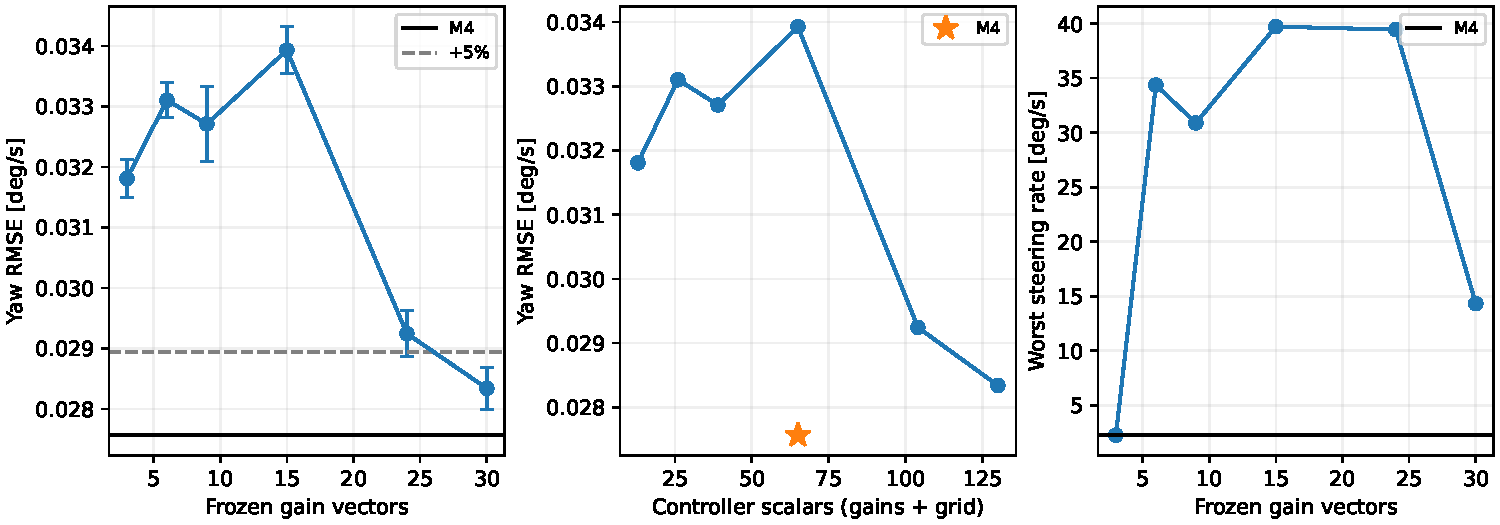
\includegraphics[width=\linewidth]{experiment_5a_complexity.pdf}
\caption{Experiment 5A: tracking versus frozen gain count and controller
storage, followed by peak steering rate. Error bars are seed standard deviations.
The horizontal tolerance line represents 5\% above M4's mean tracking error.}
\label{fig:experiment5a}
\end{figure}

The ten-anchor grid's steering RMS is 0.80576 degrees, nearly equal to M4's
0.80578 degrees, while peak steering rate rises from 2.29 to 14.33 degrees/s.
It makes up to 12 switches per varying-speed maneuver. At strong excitation,
the corresponding peak rates are 3.48 and 21.58 degrees/s. Comparable RMS
effort therefore does not imply comparable input smoothness.

Matching is aggregate, not universal across scenarios. With ten anchors per
family, gaps are 5.03\% on the original S-curve, 3.16\% on the shifted lane
change, and $-1.11\%$ at constant 22 m/s. The original S-curve narrowly fails
the scenario-specific 5\% interval criterion. A single 24 m/s gain already
slightly outperforms M4 on the constant-speed case. These findings reinforce
that the value of interpolation depends on the task and operating variation.

\paragraph{Decision and limitations.}
Within this frozen comparison, many more than three frozen gains are needed
to meet the aggregate tracking target, and M4 achieves smoother steering with
less controller storage than the first matching grid. The scheduling argument
is supported for the tested nearest-switching implementation. It is not a lower
bound over all LTI designs, optimized partitions, hysteretic switching, or
bumpless transfer schemes, and it proves no formal time-varying stability claim.
Phase 6 should now test where the advantage persists as structural heterogeneity
and speed range vary, before drawing a broader model-complexity conclusion.

\section{Phase 6: two-dimensional regime map}
\label{sec:phase6}

\subsection{Experiment 6A: scheduling--heterogeneity sweep}
\paragraph{Objective.}
Determine when each architecture is warranted rather than claiming that M4 is
universally best.

\paragraph{Setup.}
Scale structural separation using
\begin{equation}
 \vartheta_c(\gamma_h)=\vartheta_0+\gamma_h(\vartheta_c-\vartheta_0),
 \qquad \gamma_h\in\{0,0.5,1,1.5\},
\end{equation}
and use speed envelopes
$[18,22]$, $[15,25]$, and $[10,30]\,\mathrm{m\,s^{-1}}$. Compare M1--M4 in every
cell using model error, closed-loop performance, worst-family result, and
complexity.

\paragraph{Predeclared expectation.}
Global LTI is sufficient for low heterogeneity and narrow scheduling variation.
Global LPV dominates for broad scheduling variation but low heterogeneity.
Clustered LTI dominates for high heterogeneity over a narrow speed range. Clustered
LPV becomes necessary when both dimensions are large.

\paragraph{Planned evidence and decision gate.}
The main figure is a two-dimensional map of the best architecture and the relative
advantage of M4. The map must show coherent transitions rather than one method
winning due to numerical noise. Unexpected regions are investigated, not smoothed
away.

\paragraph{Results, interpretation, and decision.}
Pending.

\subsection{Experiment 6B: acceleration and coordinate-consistency check}
\label{sec:experiment6b}

\paragraph{Question and scope.}
Experiment 6A supports the scheduling--specialization decomposition but leaves
an explicit prescribed-speed plant approximation. Does its principal conclusion
survive a consistent lateral-momentum model, and does it persist when the speed
profiles are slowed below the illustrative acceleration target? This is a
paired transfer check with the 6A fitted models and controller gains frozen.
It does not refit on corrected-plant data or introduce acceleration scheduling
into the controller.

\paragraph{Coordinate correction.}
For the small-angle sideslip proxy used throughout this benchmark,
$\beta=v_y/v_x$, the lateral-momentum and yaw equations give
\begin{align}
 \dot v_y&=\frac{F_{yf}+F_{yr}}{m}-v_xr,\\
 \dot r&=\frac{l_fF_{yf}-l_rF_{yr}}{I_z},\\
 \dot\beta&=\frac{F_{yf}+F_{yr}}{mv_x}-r
             -\frac{\dot v_x}{v_x}\beta.
 \label{eq:6b-coordinate}
\end{align}
The final term follows by differentiating $v_y/v_x$. It vanishes at constant
speed, but is absent from the previous prescribed-speed implementation.
We retain the same small-angle slip expressions and tanh force laws, written
in lateral-velocity coordinates as
\begin{align}
 \alpha_f&=\delta-\frac{v_y+l_fr}{v_x}, &
 \alpha_r&=\frac{-v_y+l_rr}{v_x}.
\end{align}
The controller still receives $(\beta,r)$ at each sample. This coordinate check
does not replace the proxy by the exact angle $\arctan(v_y/v_x)$.

\paragraph{Three plant implementations.}
The historical implementation, denoted \texttt{legacy}, retains the 6A
frozen-speed RK4 step. A diagnostic, \texttt{beta\_noacc}, varies speed between
RK4 stages while omitting the final term in \cref{eq:6b-coordinate}. The
coordinate-consistent implementation, \texttt{vy}, integrates $(v_y,r)$ and
converts $v_y$ to $\beta$ at sampling instants. Speed is linearly interpolated
between prescribed samples during integration. Steering remains held over each
sample, and the integral state and sampled controller are unchanged. Comparing
the first two implementations isolates within-step speed variation. Comparing
the latter two isolates the coordinate term, up to integration error.

All three retain static axle loads, pure lateral tanh tires, and externally
prescribed longitudinal speed. There is no longitudinal-force allocation,
combined-slip friction constraint, or acceleration-induced load transfer.
Thus \texttt{vy} is coordinate-consistent under the existing bicycle
assumptions, not a full longitudinal--lateral vehicle model.

\paragraph{Frozen protocol and contrasts.}
The four selected cells use $\gamma_h\in\{0,1\}$ and speed envelopes
18--22 and 10--30 m/s. We load the committed 6A parameter fits for seeds
21--30 and reconstruct exactly the same M1--M4 gains. Test fleets remain
the paired held-out realizations 121--130. These are repeated conditions on
the same clients, not additional independent fleet evidence. Per-seed fit-file
hashes record the model provenance.

Each of the three held-out scenarios and three severities is run with its
original 12-second timing and with both speed and yaw reference stretched to
24 seconds. The sample time remains 0.01 seconds. This retains reference
amplitudes and speed support while halving the rate of both signals. Broad-range
peak speed acceleration decreases from 3.93 to 1.96 m/s$^2$. Stretching the yaw
reference also makes lateral tracking less demanding, so we compare architectures
and plants within each timing condition rather than attributing cross-duration
differences solely to acceleration.

Primary metrics and amplitude-feasibility limits remain those of 6A. Paired
bootstrap intervals resample ten seeds, using 10,000 draws and seed 6201.
The predeclared robustness gate requires M4 to improve moderate mean tracking
by at least 5\% over both M2 and M3 in the nominal-separation broad-envelope
\texttt{vy} condition at both durations, with positive lower confidence bounds
and amplitude feasibility at all tested severities. The four-corner
smallest-controller classification is a secondary descriptive result using
the previous 5\% upper-bound rule. The 6A frozen-speed stability audit applies
to the unchanged gains and constant-speed linearizations, but does not certify
the accelerating trajectories.

\paragraph{Validation and reproducibility.}
Constant-speed closed-loop trajectories and metrics agree with the previous
simulator to numerical precision. The corrected derivative is checked against
the coordinate transformation, and RK4 is checked against an independently
implemented lateral-momentum ODE using adaptive integration and step halving.
The complete suite passes 33 tests. The full legacy replay is also compared
against the committed 6A raw metrics before generating conclusions.
The entry point is \texttt{experiment\_6b\_acceleration\_validation.py}, with
the frozen protocol under \texttt{code/config/}. Compressed per-seed client and
profile CSVs support paired summaries and a \texttt{--summarize-only} rebuild.

\paragraph{Results and decision.}
All 259,200 client evaluations complete and pass amplitude feasibility.
The maximum absolute discrepancy in the retained legacy-replay metrics is
$7.95\times10^{-13}$, confirming reproduction of the corresponding 6A runs.
The unchanged frozen audit has worst spectral radius 0.96888. The primary
robustness gate passes at both durations, with all four paired comparisons
favoring M4 in all ten fleet pairs and all lower confidence bounds positive.

\Cref{tab:6b-tracking} gives the nominal-separation broad-envelope results.
At the original timing, corrected-plant M4 improves on M3 by 16.46\% and on
M2 by 25.02\%. At doubled duration, the reductions are 35.27\% and 44.95\%,
respectively. The 95\% paired intervals for the absolute mean differences
$J_{M3}-J_{M4}$ and $J_{M2}-J_{M4}$ are $[0.00491,0.00580]$ and
$[0.00893,0.00922]$ degrees/s at 12 seconds, and $[0.00378,0.00447]$ and
$[0.00603,0.00634]$ degrees/s at 24 seconds.

\begin{table}[htbp]
\centering
\caption{Experiment 6B: mean moderate yaw-rate tracking RMSE in degrees/s for
nominal separation and 10--30 m/s. Models and gains are identical across plant
implementations and timings. The corrected plant integrates lateral momentum.}
\label{tab:6b-tracking}
\begin{tabular}{lrrrr}
\toprule
 & \multicolumn{2}{c}{12 seconds} & \multicolumn{2}{c}{24 seconds}\\
Method & Legacy & Corrected & Legacy & Corrected\\
\midrule
M1 & 0.040306 & 0.040336 & 0.016590 & 0.016597\\
M2 & 0.036234 & 0.036246 & 0.013748 & 0.013748\\
M3 & 0.032481 & 0.032533 & 0.011676 & 0.011692\\
M4 & 0.027164 & 0.027177 & 0.007561 & 0.007568\\
\bottomrule
\end{tabular}
\end{table}

The slower references reduce absolute error for all four methods. Although
M4's relative advantages increase, its absolute advantages over M2 and M3
decrease. This is not evidence that reducing acceleration itself increases the
benefit of LPV. Both the lateral reference rate and its interaction with speed
change in this timing experiment.

\Cref{fig:6b-acceleration} shows that the three plant implementations nearly
overlap at the scale of the architecture differences. Across the four cells,
two durations, and four methods, the largest absolute relative change in
moderate mean tracking from \texttt{legacy} to \texttt{vy} is 0.1594\%.
Changing within-step speed treatment alone produces at most 0.01394\% change.
For broad-range nominal-family M4, the complete plant correction increases
mean error by 0.0484\% at 12 seconds and 0.0938\% at 24 seconds. These changes
are small but statistically resolvable in the paired simulations. They are
not zero, and are much smaller than the architecture contrasts in this study.

\begin{figure}[htbp]
\centering
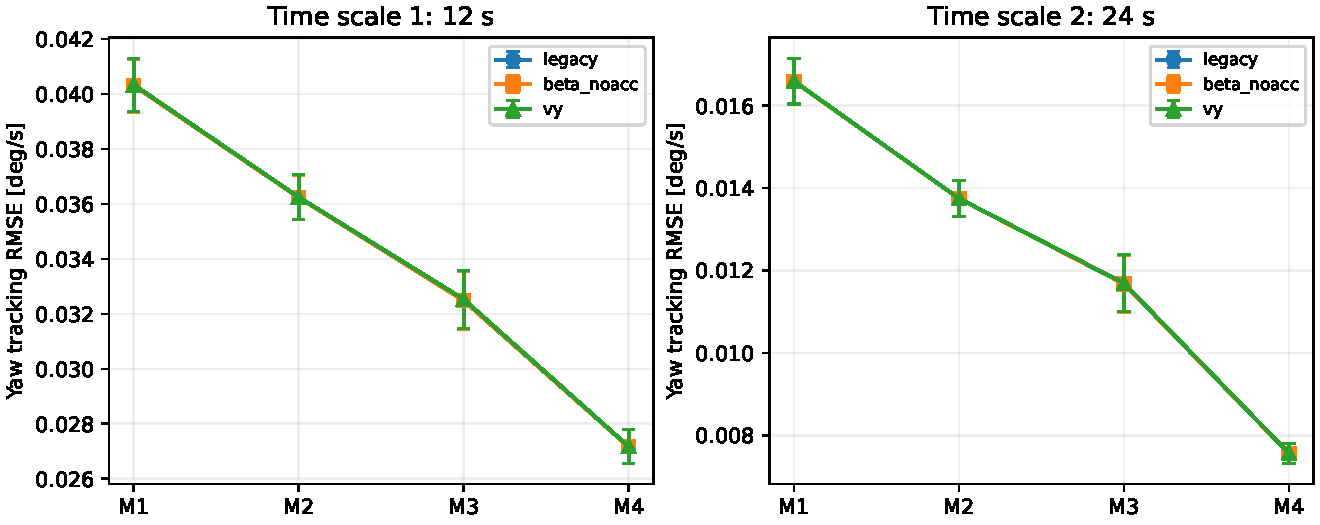
\includegraphics[width=0.95\linewidth]{experiment_6b_acceleration.pdf}
\caption{Experiment 6B: nominal-separation broad-range tracking across plant
implementations. Error bars are standard deviations across ten seed pairs.
\texttt{beta\_noacc} varies speed within RK4 but omits the coordinate term,
whereas \texttt{vy} integrates the consistent momentum equations. Their near
overlap shows that the controller-architecture differences dominate these
plant corrections under both tested timings.}
\label{fig:6b-acceleration}
\end{figure}

The four-corner descriptive classifications also remain unchanged at both
durations and for all three implementations. Global LTI is sufficient with
zero separation and narrow range, global LPV with zero separation and broad
range, family LTI with nominal separation and narrow range, and family LPV
with nominal separation and broad range. These are the corresponding four
corners of \cref{tab:6a-regimes}. The intermediate-separation and
intermediate-envelope boundaries of 6A were not rerun here.

One reason a modest effect is plausible is the size of the added term relative
to linear-tire sideslip damping. Their coefficient ratio is
\begin{equation}
 \frac{|\dot v_x|/v_x}{(C_f+C_r)/(mv_x)}
 =\frac{m|\dot v_x|}{C_f+C_r}.
\end{equation}
At the nominal center, $(C_f+C_r)/m\simeq106.7\,\mathrm{m\,s^{-2}}$, so
even the original peak speed acceleration gives approximately 3.7\% of that
linear damping coefficient. This is an explanatory scale comparison, not an
error bound for tanh tires or the closed loop. The small observed tracking
effect is established by the paired simulations.

The result supports continuing toward limited-data identification and
federation: the tested M4 advantage is not an artifact of the omitted
coordinate term or dependent on the faster timing. The remaining limitations
are the prescribed longitudinal speed, pure lateral tire model, fixed
controllers, and absence of a time-varying stability certificate. The result
does not yet validate identification on corrected-plant data or the 5A
controller-grid sweep under the new plant.

\paragraph{Implication for subsequent identification.}
The coordinate term is known kinematics shared by all clients, not a new
structural family. Identification on accelerating trajectories should either
use lateral-velocity coordinates or include the known term
$-(\dot v_x/v_x)\beta$ in its predictor. The persistent unknown parameter ratios
can then retain their original interpretation. This experiment tests transfer
of existing speed-only controllers and does not claim that the previous
identification objective is already corrected. Estimating acceleration from
noisy production signals remains a separate practical question.

\section{Phase 7: federated extension after the oracle gate}
\label{sec:phase7}
Only a positive oracle result justifies removing its assumptions. The first
federated hypothesis is deliberately narrow:
\begin{quote}
Compatible clients with complementary speed coverage can collaboratively estimate
an LPV family more accurately over the complete operating envelope than any
individual client, while family-specific aggregation prevents negative transfer.
\end{quote}
Imperfections are introduced incrementally:
\begin{enumerate}
 \item finite local data;
 \item measurement and process noise;
 \item partial and non-identical client speed coverage;
 \item local LPV estimation and uncertainty quantification;
 \item global aggregation and local-only baselines;
 \item oracle-family federated aggregation;
 \item learned family assignment;
 \item uncertainty-aware clustered aggregation;
 \item partial participation and communication limits.
\end{enumerate}
Changing payload during a drive is excluded from the first federated study. It
would make the structural state time varying and introduce change detection,
concept drift, and online reassignment before the stationary problem is understood.
Robust LPV synthesis, additional scheduling variables, and higher-fidelity vehicle
models are likewise evidence-driven later extensions.


\subsection{Experiment 7A: finite local data and the value of pooling}
\label{sec:experiment7a}

\paragraph{Question.}
The oracle results establish that persistent LPV families can be useful.
Experiment 7A asks whether the available local evidence is insufficient enough
to justify collaboration. A three-ratio physical model can potentially be
identified from a narrow speed interval. Restricted coverage alone is therefore
not assumed to create a federated-learning benefit. This experiment implements
centralized comparisons that a subsequent federated method would need to match.

\paragraph{Corrected output-error estimator.}
Let $p=(p_1,p_2,p_3)=(C_f/m,C_r/m,m/I_z)$ and $z=(v_y,r)^\top$. The linear-tire
identification model uses
\begin{equation}
 \dot z=A_z(v;p)z+B_z(p)\delta,\qquad
 \hat y=\operatorname{diag}(1/v,1)z,
\end{equation}
where
\begin{align}
 A_z(v;p)&=\begin{bmatrix}
 -(p_1+p_2)/v &(l_rp_2-l_fp_1)/v-v\\
 p_3(l_rp_2-l_fp_1)/v &-p_3(l_f^2p_1+l_r^2p_2)/v
 \end{bmatrix},\\
 B_z(p)&=\begin{bmatrix}p_1\\p_3l_fp_1\end{bmatrix}.
\end{align}
Geometry is known and unchanged. Integrating lateral velocity incorporates
the coordinate correction of \cref{sec:experiment6b}. RK4 uses linearly
interpolated speed within each sample, and measured steering is held constant.

For a set of independent records $\mathcal D$, we solve
\begin{equation}
 \hat p=\arg\min_{p>0}\sum_{d\in\mathcal D}\sum_{k=1}^{N_d}
 \left\|W\big(\hat y_{d,k}(p)-y_{d,k}\big)\right\|_2^2,
 \qquad W=\operatorname{diag}(1/s_\beta,1/s_r),
\end{equation}
with $s_\beta=0.05$ degrees and $s_r=0.1$ degrees/s, converted to radians in
the implementation. These scales remain fixed in the clean-data comparisons.
Every simulated record starts from the known zero state. The predictor
propagates from that state throughout the record and does not reset to noisy
measured states. Thus measurement noise in the output is not inserted as an
exact state regressor, as it would be in a naive one-step least-squares fit.

The positive log-parameter optimization retains the 4F bounds
$[1,1,0.05]\leq p\leq[300,300,3]$ and two initial guesses
$(40,40,0.5)$ and $(80,60,1)$. The lowest training objective selects the solution.
All three stopping tolerances are $10^{-9}$, with 150 function evaluations per
start. Complex-step derivatives and a banded solve of the linear state
recurrence accelerate computation without changing the objective. Fit status,
active bounds, differences between starts, and the column-scaled Jacobian
condition number are retained. The latter is a sensitivity diagnostic, not a
calibrated confidence interval under nonlinear model mismatch.

\paragraph{Factorial data protocol.}
Ten new fleet realizations, seeds 31--40, each contain ten clients in each of
the three nominal-separation families. Every client contributes three separate
constant-speed episodes. This avoids confounding a short recording budget
with an unrealistically rapid traversal of the full speed envelope. Broad
coverage uses speeds $(10,20,30)$ m/s. Restricted coverage assigns each client
one of the three anchor sets $(10,14,18)$, $(16,20,24)$, or $(22,26,30)$ m/s.
Their interval hulls overlap, although the observations are at discrete anchors.
Each family receives the same category counts, with a seed-dependent random
assignment to client indices. Scheduling coverage is therefore not a proxy
for the family label.

Episode durations are 2 and 8 seconds, giving total local data budgets of
6 and 24 seconds. Short records are prefixes of the corresponding long records.
The three yaw references have the fixed form
\begin{equation}
 r_j^\star(t)=3\frac{\pi}{180}(1-e^{-t/0.3})
                 \sin(2\pi\,0.35t+0.7j),\qquad j=0,1,2.
\end{equation}
A single nominal global scheduled controller collects all records on the
corrected tanh-tire plant. Its parameters are the nominal center ratios, and
its gains use the existing common LQI weights. It does not use true family
labels or individual parameters to adapt collection. Identification labels
are supplied only for the oracle-family pooling comparison.

Noise-free outputs are compared with independent Gaussian noise of standard
deviation 0.05 degrees on the sideslip proxy and 0.1 degrees/s on yaw rate.
These are declared synthetic measurement assumptions, not calibrated sensor
specifications. The same standardized noise draws are reused across coverage
conditions and record prefixes. Noise is added to the identification records,
not to the data-collection feedback. Steering and speed are exact, process
noise is absent, and the initial state is known. Availability of a sideslip
measurement or sufficiently reliable estimate remains an idealization.

\paragraph{Three comparisons and data accounting.}
\textbf{Local} fits one model per client using only that client's records.
\textbf{Global} fits one model to all 30 clients' available records.
\textbf{Family} fits three models using the oracle labels, ten clients per fit.
All use the same estimator, bounds, and available dataset for a given cell.
Pooling intentionally provides additional data: in the short condition, the
local, family, and global fits use 6, 60, and 180 seconds, respectively.
The long-data local fit supplies a reference for how additional individual
evidence changes the comparison. The experiment does not claim a pooling
benefit at equal total sample count per fitted model.

All models generate speed-scheduled LQI controllers on the common five-point
10--30 m/s grid with the previous fixed weights. Local fitting deploys 30
model/controller families, oracle-family pooling three, and global pooling one.
No controller weight, model choice, or data condition is selected on test error.
This is batch nonlinear least squares, with neither RLS nor federated messages
nor learned clustering.

\paragraph{Held-out evaluation and decision rule.}
Each physical client is evaluated on the three held-out 24-second moderate
trajectories from 6B, covering varying speed and an unseen constant speed.
Training and test trajectories are separate. The evaluated clients are the
same physical systems that supplied the local data, which is necessary to
assess their personalized fits. The ten fleet realizations, not individual
clients or scenarios, are the independent statistical units.

We report yaw tracking RMSE, worst-family tracking, steering RMS and peak rate,
amplitude feasibility, and the 161-speed frozen audit. Common-input free-run
prediction is evaluated separately on test trajectories collected by the
nominal controller, so every candidate predicts the same steering sequence.
Separate sideslip and yaw errors are retained, alongside relative error in
the three true parameter ratios for diagnostic use only. The nonlinear plant
is not exactly representable by the fitted linear-tire model.

The predeclared primary cell is short, noisy, restricted coverage. The
collaboration gate requires oracle-family pooling to reduce mean tracking
error relative to Local by at least 5\%, with a positive lower paired
bootstrap bound, family-controller amplitude feasibility, and frozen radius
below one. Bootstrap intervals use ten fleet seeds, 10,000 draws, and seed
7101. Global pooling, other cells, worst-family errors, and prediction errors
explain the result but do not replace a failed primary gate.

\paragraph{Results, interpretation, and next decision.}
All 2,720 fits converge from both starts, with no bound hits; the largest
column-scaled Jacobian condition number is 10.49 and the largest relative
multistart parameter difference is $1.14\times10^{-7}$. All 21,600 closed-loop
evaluations satisfy amplitude feasibility. The maximum frozen spectral radius
is 0.96931; this remains a frozen audit, not a varying-speed stability proof.

\begin{table}[htbp]
\centering
\caption{Experiment 7A primary cell: six seconds per client, noisy outputs,
restricted coverage. Tracking is mean $\pm$ sample standard deviation across
ten fleets. Prediction uses common held-out inputs. Parameter error is the
root mean square of the three componentwise relative errors.}
\label{tab:experiment7a}
\begin{tabular}{lrrrr}
\toprule
Method & Families & Tracking [deg/s] & Yaw prediction [deg/s] & Parameter error\\
\midrule
Local & 30 & $0.006681\pm0.000041$ & 0.04710 & 0.82\%\\
Family & 3 & $0.007457\pm0.000105$ & 0.14067 & 2.52\%\\
Global & 1 & $0.011713\pm0.000590$ & 0.35905 & 7.66\%\\
\bottomrule
\end{tabular}
\end{table}

\begin{figure}[htbp]
\centering
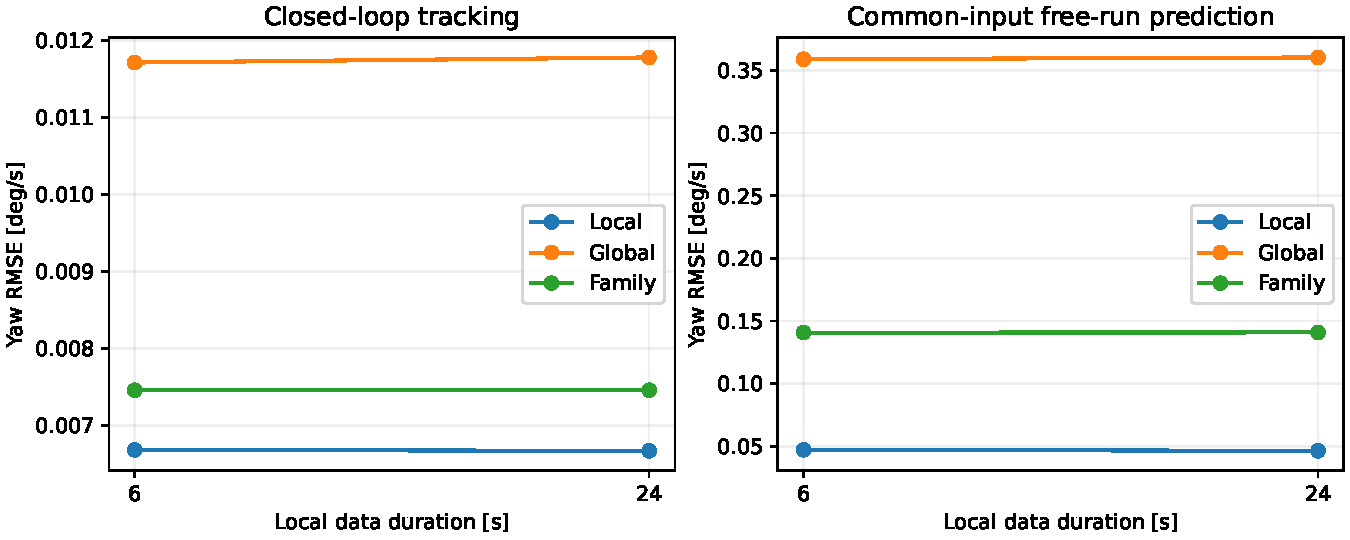
\includegraphics[width=\linewidth]{../results/figures/experiment_7a_local_identification.pdf}
\caption{Experiment 7A: noisy restricted-coverage results as local recording
duration increases. Closed-loop tracking and common-input prediction are
different evaluations; their absolute errors should not be equated.}
\label{fig:experiment7a}
\end{figure}

As shown in \cref{tab:experiment7a,fig:experiment7a}, family pooling increases
primary tracking error by 11.62\% relative to Local. The paired difference
$J_{\rm Local}-J_{\rm Family}$ is $-0.000776$ deg/s, with 95\% paired bootstrap
interval $[-0.000836,-0.000714]$ deg/s. None of the ten fleet pairs favors
Family. The predeclared collaboration gate therefore fails. Family pooling
does improve tracking by 36.33\% relative to Global, but this secondary
comparison cannot replace the failed Local comparison.

Local also has lower mean tracking error in all eight data conditions.
For short restricted records, removing measurement noise changes Local
tracking from 0.006681 to 0.006674 deg/s and its parameter error from 0.82\%
to 0.21\%. Extending noisy restricted records from six to 24 seconds lowers
Local parameter error to 0.41\%, but barely changes tracking (0.006669 deg/s).
Family tracking remains approximately 0.007457 deg/s. Thus local estimation
variance is already small in the tested regime. The physical three-ratio
structure permits generalization beyond a client's measured speed anchors;
restricted coverage does not by itself create a substantial information gap.
The persistence of the pooling penalty with clean and longer records supports
within-family approximation bias as the dominant explanation here. Nonlinear
model mismatch remains present, so this is evidence from controlled contrasts,
not an exact bias--variance decomposition.

The primary worst-family tracking errors are 0.006823, 0.007817, and 0.013517
deg/s for Local, Family, and Global, respectively. Steering RMS is approximately
0.80961 degrees for all three, with peak rates approximately 1.163 degrees/s.
The ordering is therefore not explained by a large steering-effort difference.
Family deploys three scheduled families instead of Local's 30, at an 11.62\%
relative tracking penalty (0.000776 deg/s absolute). This is a measurable
complexity--performance trade-off, not evidence that collaboration improves
individual prediction or tracking accuracy.

\paragraph{Consequence for the next experiment.}
Do not proceed to federated optimization with a claim that its accuracy benefit
has already been established. A useful next diagnostic is a predeclared
personalization comparison: local fitting, fixed oracle-family pooling, and
family-informed local regularization, with regularization chosen using training
validation only. This would test whether sharing can reduce uncertainty while
retaining client-specific differences. Any harder data regime must be motivated
independently and specified before testing, rather than increasing noise until
pooling wins. Learned clustering and decentralized optimization remain later
questions. The negative 7A gate is retained regardless of subsequent outcomes.

\paragraph{Reproducibility.}
The frozen protocol is \texttt{code/config/experiment\_7a.json}; the runner is
\texttt{code/experiments/experiment\_7a\_local\_identification.py}.
Per-seed compressed tables retain client metrics, fitted parameters, prediction
errors, and data manifests. Summary tables, paired comparisons, and the gate
decision are stored under \texttt{results/tables/experiment\_7a*}.
The \texttt{--summarize-only} option regenerates aggregate evidence without
refitting. Predictor integration, record resets, exact-parameter recovery,
and client-specific controller dispatch are covered by regression checks;
the complete suite contains 36 passing tests.

\subsection{Experiment 7B: family-informed personalization}
\label{sec:experiment7b}

\paragraph{Reason for the revised sequence.}
Experiment 7A fails the collaboration gate because accurate local fits
outperform fixed family pooling. Consequently, the originally envisaged next
step of federated estimation is deferred. Experiment 7B instead tests the
personalization diagnostic proposed in \cref{sec:experiment7a}: can a family
prior help local estimation without forcing different clients to share the
same parameters? The failed 7A result is retained. This experiment remains
centralized and uses oracle family labels.

\paragraph{Unchanged data regime and new fleets.}
The protocol uses ten new realizations, seeds 41--50, with 30 clients each.
It retains the primary 7A regime: three two-second constant-speed episodes,
restricted speed anchors, sideslip-proxy noise of 0.05 degrees, and yaw-rate
noise of 0.1 degrees/s. Family separation, client scatter, nominal collection
controller, references, known initial state, and exact speed and steering are
unchanged. Neither noise nor scarcity is increased after observing 7A.
The same three held-out 24-second scenarios and corrected tanh-tire plant are
used for evaluation. These fleets are independent of 7A; within each fleet,
test trajectories belong to the same physical clients as identification.

\paragraph{Family prior without validation leakage.}
For client $i$, first fit $\bar p_{c,-i}$ using only the other nine members
of its true family. No record from client $i$ contributes to this prior.
This gives a fixed donor prior for all of the client's validation folds.
Using the 7A output predictor and scales, the personalized estimate is
\begin{equation}
 \hat p_i(\lambda;\mathcal D)=\arg\min_{p\in\mathcal P}
 \frac{1}{2N_{\mathcal D}}\sum_{d,k}
 \left\|W\big(\hat y_{d,k}(p)-y_{d,k}\big)\right\|_2^2
 +\lambda\left\|\frac{\log p-\log\bar p_{c,-i}}{0.05}\right\|_2^2,
 \label{eq:7bobjective}
\end{equation}
where $N_{\mathcal D}$ counts transitions, so $2N_{\mathcal D}$ counts scalar
output residuals. The logarithm acts componentwise and $\mathcal P$ is the
same positive bounded parameter domain as in 7A. The fixed 0.05 log scale
sets the penalty units; it is not an estimated prior standard deviation.
Normalizing the data term makes the meaning of $\lambda$ consistent between
four-second fold fits and the six-second final fit. The implementation
multiplies the whole objective by the number of scalar residuals and appends
the resulting prior residuals to the least-squares problem. At $\lambda=0$,
it exactly preserves the unregularized fitting objective and implementation.
Both solver starts and tolerances are unchanged.

\paragraph{Selection using identification records only.}
The candidate strengths are fixed before execution:
\begin{equation}
 \Lambda=\{0,10^{-3},10^{-2},10^{-1},1,10\}.
\end{equation}
For each candidate, fit on two complete episodes and predict the third from
its known zero initial state. Repeat for all three held-out episodes and
select the smallest average standardized output error. Ties select the lower
strength. This validates free-run prediction, not closed-loop tracking.
The selected strength is then used to refit on all three local episodes.
If zero is selected, the final Local fit is reused exactly. No additional
validation recordings are supplied and no test trajectory, true parameter,
or test tracking metric enters selection. Since validation episodes contain
different speed anchors, the selection also probes prediction beyond the
two fitting anchors within the client's assigned interval.

\paragraph{Comparisons and resource accounting.}
\textbf{Local} fits all six seconds from each client independently.
\textbf{Family} fits one shared model to all ten clients' six-second records
in each true family. \textbf{Personalized} uses the donor prior and selected
local estimate in \cref{eq:7bobjective}. Family pooling remains an exact
comparison to the deployed family architecture in 7A, whereas the prior
excludes the recipient specifically to protect validation integrity.
All methods access the same recorded fleet dataset. Each donor prior uses
54 seconds, each Family fit 60 seconds, and each Local final fit six seconds.
Each validation candidate uses four local seconds for fitting and two for
scoring. Personalization increases fitting effort and deploys 30 model and
controller families, just as Local does; it does not inherit Family's
three-family deployment advantage. The leave-one-client-out priors are a
diagnostic construction, not an efficient federated implementation.

\paragraph{Evaluation and decision rule.}
The common LQI weights, gain grid, held-out prediction inputs, amplitude
checks, and 161-speed frozen audit are retained. The primary gate requires
Personalized to improve fleet-average tracking relative to Local by at least
5\%, with a positive lower 95\% paired bootstrap bound, amplitude feasibility,
and frozen spectral radius below one. The ten fleet seeds are the independent
units; bootstrap uses 10,000 draws and seed 7201. Comparisons against Family,
worst-family tracking, parameter error, common-input prediction, and selected
strength counts are secondary diagnostics. Lower cross-validation error alone
does not constitute held-out improvement, since it is the selection objective.

\paragraph{Results and interpretation.}
All 6,284 fits, including the 5,400 validation fits, converge from both starts
without bound hits. Final fits are reused for the 46 clients selecting zero
regularization. The maximum multistart relative parameter difference is
$4.44\times10^{-7}$. All 2,700 closed-loop evaluations satisfy amplitude
limits and the largest frozen spectral radius is 0.96933. These checks do not
constitute a formal varying-speed stability guarantee.

\begin{table}[htbp]
\centering
\caption{Experiment 7B on ten new fleets: six seconds of noisy restricted
local data. Tracking reports mean $\pm$ standard deviation across fleet seeds.
Parameter error uses the same componentwise relative-error convention as 7A.}
\label{tab:experiment7b}
\begin{tabular}{lrrr}
\toprule
Method & Tracking [deg/s] & Yaw prediction [deg/s] & Parameter error\\
\midrule
Local & $0.006669\pm0.000016$ & 0.04667 & 0.787\%\\
Family & $0.007651\pm0.000368$ & 0.15837 & 2.627\%\\
Personalized & $0.006672\pm0.000017$ & 0.04637 & 0.842\%\\
\bottomrule
\end{tabular}
\end{table}

\begin{figure}[htbp]
\centering
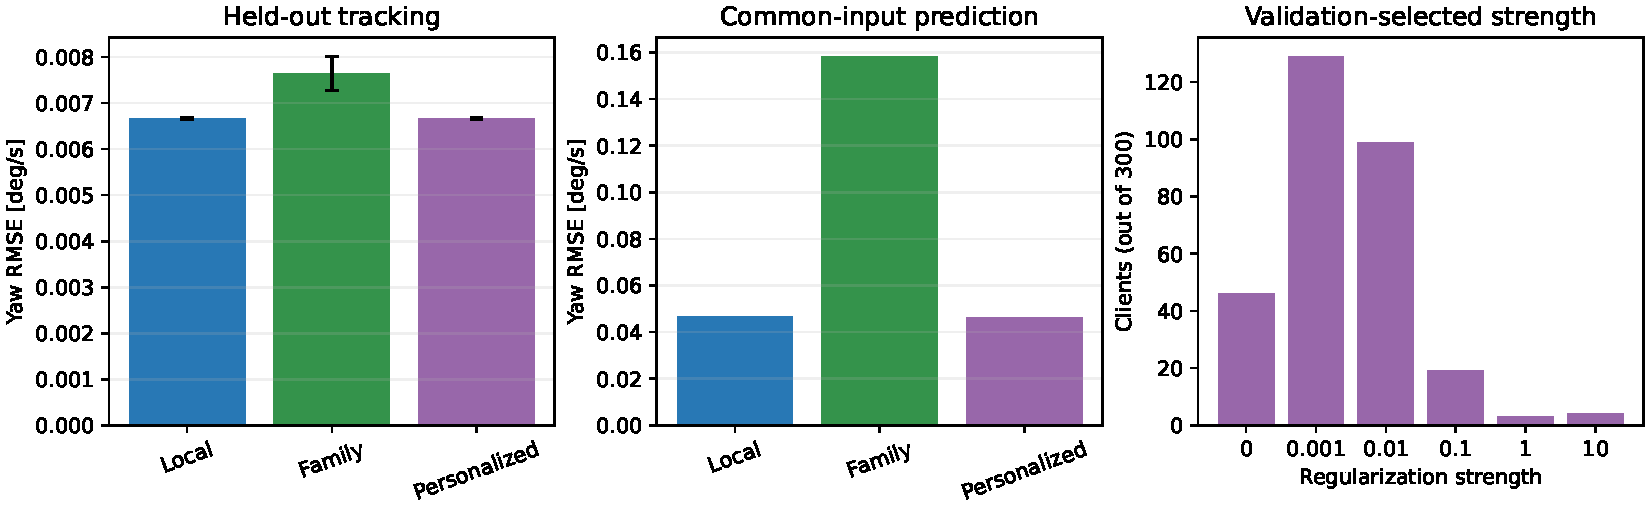
\includegraphics[width=\linewidth]{../results/figures/experiment_7b_personalization.pdf}
\caption{Experiment 7B: held-out tracking, common-input yaw prediction, and
the distribution of validation-selected regularization strengths. Tracking
error bars show standard deviation across ten fleets. Prediction and tracking
use different inputs and should not be compared in absolute magnitude.}
\label{fig:experiment7b}
\end{figure}

\Cref{tab:experiment7b,fig:experiment7b} shows that personalization nearly
recovers Local performance while improving tracking over Family by 12.79\%.
Against Local, however, tracking error increases by 0.0573\%. The paired
difference $J_{\rm Local}-J_{\rm Personalized}$ is
$-3.82\times10^{-6}$ deg/s, with 95\% bootstrap interval
$[-7.37\times10^{-6},-1.65\times10^{-7}]$ deg/s. Three of ten fleet pairs
favor Personalized. The primary 5\% improvement gate therefore fails.
The absolute penalty is tiny, so the practical conclusion is near-parity,
with no demonstrated tracking improvement, rather than a substantial
personalization failure.

The selected-strength counts for $\lambda=0,0.001,0.01,0.1,1,10$ are
46, 129, 99, 19, 3, and 4, respectively. Thus 274 of 300 clients select at
most 0.01. This supports weak shrinkage in this setting; it does not show
that those strengths are optimal outside the tested grid or data regime.
The four upper-end selections are retained without expanding the grid after
seeing test outcomes. Common-input yaw prediction improves by only 0.64\%
relative to Local, with paired difference interval
$[-0.000187,0.000808]$ deg/s spanning zero. Relative parameter error increases
from 0.787\% to 0.842\%. Neither secondary result establishes a reliable
estimation advantage. Worst-family tracking is likewise nearly unchanged,
0.006805 versus 0.006808 deg/s. Steering RMS is approximately 0.80852 degrees
for both, with peak rates about 1.1693 degrees/s.

\paragraph{What this establishes and what remains open.}
Forcing all family members to use one estimate causes a measurable penalty,
and allowing local parameters largely removes it. Nevertheless, the strong
three-ratio structure and available state observations already allow accurate
local identification. A donor prior has little estimation uncertainty to
remove here, while it can still introduce client mismatch. This interpretation
is consistent with 7A's clean-data and data-length contrasts, although 7B does
not provide a formal bias--variance decomposition. Prediction-based validation
also need not minimize downstream tracking error.

Experiments 7A and 7B therefore do not yet justify a claim of federated accuracy
improvement. Fixed family sharing has a deployment-complexity trade-off;
personalization retains 30 controllers and recovers local accuracy. Those are
distinct findings. The next decision should be whether the intended application
actually has a local information limitation absent here, such as unavailable
sideslip measurements or insufficient excitation. Such an assumption must be
motivated and specified before a new experiment. Further tuning of this
regularization grid or increasing noise solely to obtain a positive result
is not the default next step. Federated optimization and learned clustering
remain deferred.

\paragraph{Reproducibility.}
The protocol is \path{code/config/experiment_7b.json}. The runner is:
\begin{quote}\small
\path{code/experiments/experiment_7b_personalization.py}
\end{quote}
Set \texttt{PYTHONPATH=code/src}. The \texttt{--summarize-only} option rebuilds
the aggregates and figure. Compressed per-seed outputs retain every fold's
candidate parameters, validation loss and solver diagnostics, selected strengths,
final fits, donor identities, identification-data hashes, and held-out metrics.
The conclusions file records protocol and implementation hashes.
The 38-test suite includes exact preservation at zero regularization, approach
to the prior under a dominant penalty, explicit episode exclusion in validation,
and rejection of an incorrect prior on clean identifiable data.

\subsection{Experiment 7C: complementary local operating coverage}
\label{sec:experiment7c}

\paragraph{Question and frozen gate.}
Experiments 7A and 7B show that six seconds over three nearby speeds already
suffice for accurate local structured identification. Experiment 7C therefore
tests the more restrictive premise needed by the federated argument: can
compatible clients compensate for operating regions that a recipient never
observes? The primary gate requires oracle Family pooling to reduce mean
held-out tracking error relative to Local by at least 5\%, with a positive
lower 95\% paired-seed bootstrap bound, amplitude feasibility, and maximum
frozen spectral radius below one. The gate and protocol were fixed before the
ten new fleets (seeds 51--60) were evaluated.

\paragraph{Complementary data and controls.}
Each of the ten clients in an oracle family is assigned one constant collection
speed from $\{10,12,14,16,18,22,24,26,28,30\}$ m/s and records three independent
one-second steering episodes only at that speed. Thus a Local fit receives 300
transitions from a single speed, whereas a Family fit receives 3,000 transitions
whose union covers the full envelope. Global pools all three families. As an
information-budget control, LocalExtra gives every recipient 3,000 transitions
collected from that same vehicle over all ten speeds. It is an oracle for the
value of additional local calibration, not a deployable federated method.
All fits use the unchanged bounded three-ratio output-error estimator, noise
levels, controller synthesis, three 24-second held-out scenarios, amplitude
checks, and 161-speed frozen stability audit. Test trajectories are generated
only after identification. No test metric enters model fitting or selection.

\paragraph{Results.}
All 640 fits converge from both starts without bound hits; the largest relative
multistart difference is $2.46\times10^{-7}$. All 3,600 closed-loop evaluations
are amplitude-feasible and the maximum frozen spectral radius is 0.96938.

\begin{table}[htbp]
\centering
\caption{Experiment 7C on ten new fleets. Tracking reports mean $\pm$ sample
standard deviation across fleet seeds. Parameter error is componentwise relative
error. LocalExtra has the same transition count as Family but uses recipient-local
full-envelope data.}
\label{tab:experiment7c}
\begin{tabular}{lrrr}
\toprule
Method & Tracking [deg/s] & Yaw prediction [deg/s] & Parameter error\\
\midrule
Local & $0.006703\pm0.000052$ & 0.04931 & 1.499\%\\
Global & $0.011755\pm0.000465$ & 0.36889 & 7.383\%\\
Family & $0.007615\pm0.000127$ & 0.15873 & 2.617\%\\
LocalExtra & $0.006683\pm0.000051$ & 0.04792 & 0.478\%\\
\bottomrule
\end{tabular}
\end{table}

\begin{figure}[htbp]
\centering
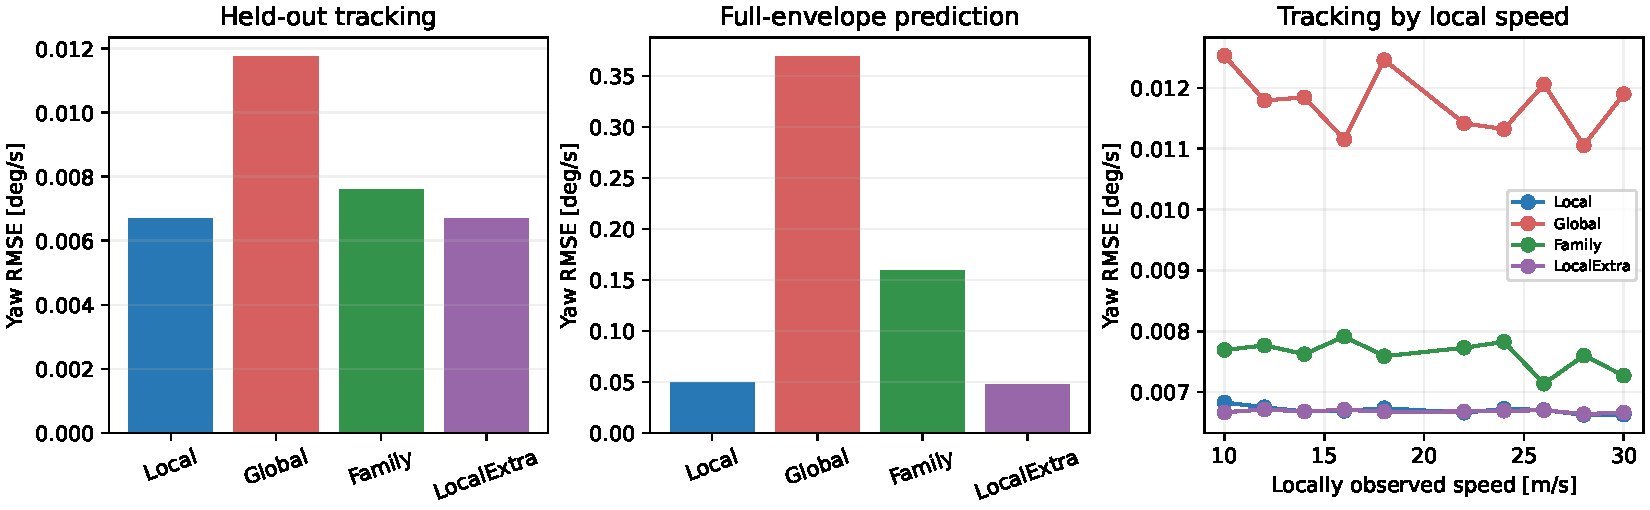
\includegraphics[width=\linewidth]{../results/figures/experiment_7c_complementary_coverage.pdf}
\caption{Experiment 7C held-out tracking, full-envelope common-input prediction,
and tracking grouped by the client's single observed speed. Tracking error bars
in the first panel show standard deviation across ten fleets.}
\label{fig:experiment7c}
\end{figure}

\Cref{tab:experiment7c,fig:experiment7c} shows that Family pooling improves
tracking by 35.22\% relative to Global, with all ten paired fleets favorable.
It nevertheless increases tracking error by 13.61\% relative to Local. The
paired difference $J_{\rm Local}-J_{\rm Family}$ is
$-9.12\times10^{-4}$ deg/s, with 95\% bootstrap interval
$[-9.76\times10^{-4},-8.49\times10^{-4}]$ deg/s; none of the ten pairs favors
Family. The primary collaboration gate therefore fails. Family also has
221.91\% higher yaw-prediction error and 74.56\% higher relative parameter
error than Local. LocalExtra slightly improves tracking over Local and reduces
parameter error to 0.478\%, confirming that additional informative local data
remain useful even though their effect on closed-loop tracking is small.

\paragraph{Interpretation and decision.}
Complementary speed coverage is not the missing condition in this benchmark.
The known three-ratio bicycle structure lets a single-speed, three-second local
record identify a controller-relevant model accurately enough to extrapolate
over the full envelope. Pooling supplies speeds but also averages persistent
within-family parameter differences; here that bias is larger than the variance
removed by collaboration. The result is especially informative because it is
not caused by instability, infeasibility, an unlucky seed, or unequal data in
the Family--LocalExtra comparison.

Together, 7A--7C reject the current federated-accuracy route based only on finite
data, nearby-speed restriction, personalization, or complementary speed coverage.
An actual federated optimizer would approximate a centralized Family solution
whose accuracy gate has now failed repeatedly, so implementing it cannot repair
the statistical premise. The project should retain the oracle scheduling--
heterogeneity contribution and the negative sharing boundary. A further FL
study is justified only by a qualitatively different and application-grounded
information constraint, such as missing state labels, excitation directions
that make the local ratios unidentifiable, or a communication/deployment goal
that does not claim improved accuracy.

\paragraph{Reproducibility.}
The frozen protocol is \path{code/config/experiment_7c.json}. The runner is:
\begin{quote}\small
\path{code/experiments/experiment_7c_complementary_coverage.py}
\end{quote}
Set \texttt{PYTHONPATH} to \path{code/src:code/experiments}. The
\texttt{--summarize-only}
option rebuilds all aggregate tables and the figure. Compressed per-seed files
retain client metrics, fit diagnostics, prediction errors, local-speed assignments,
and transition-budget accounting. The conclusions file records hashes of the
protocol, runner, and estimator.

\section{Path to paper consolidation}
During development, this report favors traceability over page limits. Failed
experiments, revised assumptions, and negative findings remain documented. Paper
consolidation begins only after the oracle gates and at least one convincing
non-oracle federated result.

The consolidated paper should center on one precise claim and retain only the
decisive evidence. A likely structure is: problem and motivation, proposed
federated LPV method, experimental methodology, decisive oracle result, federated
result under partial operating coverage, limitations, and conclusion. Candidate
contributions are the scheduling--structure decomposition, an uncertainty-aware
clustered federated LPV identification method, and evidence that a small number of
LPV families replaces many frozen LTI regimes. The development report remains the
complete experimental record and supplies supplementary details.

\section{Current execution status}
The repository scaffold and initial continuous-time bicycle model are available.
The next executable task is Experiment~0A. Identification trajectories,
controllers, and federated learning are intentionally blocked until the nominal
plant, discretization, handling behavior, and operating envelope pass that audit.

\section{Experiment 8A: paper-readiness and contribution audit}
\label{sec:experiment8a}

\paragraph{Purpose.}
Experiment 8A is a scope and evidence audit rather than another performance
benchmark. It asks which claims survive the complete sequence through 7C, what
the paper can be about without overstating federation, and which checks remain
necessary before freezing a manuscript. The audit treats failed gates as
evidence and does not redefine success criteria after seeing results. Its frozen
record is \path{code/config/experiment_8a.json}; the machine-readable claim map
is \path{results/tables/experiment_8a_claim_audit.csv}.

\paragraph{Decision.}
The project is \emph{conditionally ready as an LPV identification and control
paper}, but it is not ready as a federated-algorithm paper. The proposed central
claim is:
\begin{quote}
Measurable operating variation and persistent fleet heterogeneity are distinct
design axes: scheduling addresses the former, whereas model specialization
addresses the latter. Their combination is needed only when both effects are
large enough relative to the required control accuracy.
\end{quote}
This is an empirical design rule within the tested benchmark, not a universal
theorem. The paper should use ``fleet'' or ``multi-system'' rather than
``federated'' in its title unless a later experiment supplies an actual
distributed method and a separately justified benefit.

\begin{table}[htbp]
\centering
\caption{Experiment 8A claim audit. ``Boundary'' denotes a supported negative
or limiting result rather than a positive method contribution.}
\label{tab:experiment8a-claims}
\begin{tabular}{p{0.08\linewidth}p{0.44\linewidth}p{0.18\linewidth}p{0.16\linewidth}}
\toprule
ID & Candidate claim & Status & Evidence\\
\midrule
C1 & Scheduling and specialization address different variation axes & Primary, supported & 2, 3, 4G, 6A, 6B\\
C2 & Structured family LPV identification enables redesign on nonlinear-plant data & Supported & 4F, 4G, 6B\\
C3 & Scheduled M4 uses fewer stored gains than the matching tested LTI grid & Supported with scope & 5A\\
C4 & Family sharing beats Global but need not beat accurate Local identification & Boundary, supported & 7A--7C\\
C5 & A federated LPV algorithm improves accuracy or control & Unsupported & None\\
\bottomrule
\end{tabular}
\end{table}

\paragraph{Defensible contributions.}
The first contribution is the two-axis regime map. Experiment 6A varies speed
envelope and family separation independently and recovers the four expected
architectures: Global LTI, Global LPV, Family LTI, and Family LPV. Experiment 6B
preserves the corner decisions under corrected varying-speed dynamics and slower
maneuvers. The second contribution is methodological: unconstrained matrix
regression on nonlinear-plant records can yield unsuitable control redesigns,
whereas the structured positive parameter-ratio estimator restores the intended
family LPV advantage and transfers across independent fleets and trajectories
in 4F--4G. The third is a bounded implementation result: in the tested search,
M4 stores 15 gain vectors while the first gridded family-LTI alternative meeting
the 5\% tracking tolerance stores 30. The fourth is a boundary result:
Experiments 7A--7C consistently show that oracle-family sharing reduces error
relative to Global pooling but cannot outperform a highly data-efficient Local
structured fit.

\paragraph{Claims explicitly excluded.}
The present evidence does not support federated optimization, learned clustering,
privacy preservation, communication efficiency, online adaptation, formal
closed-loop stability, a universal model-selection law, or general superiority
of LPV control. Frozen-radius audits and amplitude feasibility are empirical
checks, not stability proofs. The complexity comparison is conditional on the
tested gain grids and switching rule. Results use synthetic vehicle families,
prescribed longitudinal speed, pure lateral tire forces, known scheduling, and
measured sideslip proxy and yaw rate.

\paragraph{Minimum work before manuscript freeze.}
Only three items are classified as required. First, independently regenerate
the headline numbers and figures from saved configurations and verify that every
paper value traces to an artifact. Second, add one targeted higher-fidelity
robustness check that introduces a genuinely absent coupling, preferably
longitudinal dynamics with combined-slip tire forces; this should test the
regime-map conclusion rather than launch a new method search. Third, sharpen the
baseline and literature comparison against established local-LPV and multi-model
identification/control approaches. Real vehicle data, learned family assignment,
formal robust synthesis, and communication studies would strengthen the work but
are not prerequisites for the scoped simulation paper.

\paragraph{Candidate manuscript blueprint.}
The recommended title is \emph{Scheduling or Specialization? Structured LPV
Identification and Control under Operating and Fleet Heterogeneity}. After the
introduction, the paper should define the two variation axes and four candidate
architectures, present the nonlinear benchmark and structured estimator, report
the regime map and robustness result, then give the redesign and complexity
evidence. A compact final subsection should report 7A--7C as the boundary of
collaboration: model sharing is valuable relative to a global model and for
model-count reduction, but does not improve accuracy over Local here. The full
diagnostic path, including failed 4D and 4D-R designs, belongs in supplementary
material rather than the main narrative.

\paragraph{Decision on an FL extension.}
The current manuscript should not be delayed by implementing distributed
optimization of the failed Family objective. Any FL extension starts with a new
oracle mechanism and an application-grounded benefit. It enters this paper only
if that gate adds a result that materially changes the contribution; otherwise
it should become a separate study. This separation protects both stories: the
LPV paper remains evidence-complete, while a future FL method is judged against
Local rather than only against an intentionally weak Global baseline.

\section{Experiment 8B: federated-equivalence and secure-aggregation gate}
\label{sec:experiment8b}

\paragraph{Purpose and scope.}
Experiment 8B implements the first actual federated estimator in this project.
Its purpose is deliberately limited: establish that the structured output-error
objective can be optimized without transmitting trajectories and that an
aggregate-only message path preserves the centralized solution before privacy
noise is introduced. It does not revisit the failed Family-versus-Local accuracy
gate and does not claim that secure aggregation is differential privacy.

\paragraph{Distributed objective.}
For a candidate log-parameter vector $q=\log p$, client $i$ evaluates its local
standardized output-error residual $e_i(q)$ and complex-step Jacobian $J_i(q)$.
It returns only
\begin{equation}
 m_i(q)=\begin{bmatrix}\tfrac12 e_i(q)^\top e_i(q) &
 J_i(q)^\top e_i(q)\end{bmatrix}^\top\in\mathbb R^4.
\end{equation}
The server sums these messages to obtain the pooled objective and gradient and
updates the three log parameters with bounded L-BFGS-B. The server broadcasts
three candidate parameters per evaluation. Two fixed initializations are used,
matching the centralized estimator's multistart principle. Global aggregation
uses all 30 clients; oracle-Family aggregation runs independently for each group
of ten. The data protocol otherwise repeats 7C on fresh fleets, seeds 61--70.

\paragraph{Aggregate-only emulator and threat boundary.}
The Secure path adds deterministic pairwise random masks to the four-number
client messages; masks cancel only in the sum. This numerically emulates what the
server-side optimizer receives under secure aggregation. It is not a production
cryptographic protocol, provides no implementation-level security claim, and
does not handle client dropout or collusion. Floating-point mask cancellation
can change the optimizer path at roundoff level. Consequently, the absolute
Secure--Federated parameter tolerance is $10^{-6}$; an earlier $10^{-10}$ audit
threshold was corrected because it incorrectly treated floating-point emulation
as exact fixed-point cryptographic arithmetic. This correction changes only the
equivalence audit, not any fitted model or performance result.

\paragraph{Gate and results.}
The gate requires convergence, centralized--federated relative parameter error
below $2\times10^{-4}$, tracking difference below $10^{-5}$ deg/s,
Secure--Federated absolute parameter difference below $10^{-6}$, amplitude
feasibility, and maximum frozen spectral radius below one. All conditions pass.
All 120 fits converge and all 5,400 evaluations are feasible. The maximum
centralized--federated relative parameter discrepancy is
$7.65\times10^{-8}$; the maximum tracking discrepancy is
$6.12\times10^{-10}$ deg/s. The maximum Secure--Federated parameter difference
is $4.42\times10^{-7}$, and the largest frozen spectral radius is 0.96876.

\begin{table}[htbp]
\centering
\caption{Experiment 8B tracking results across ten fresh fleets. Values are
mean $\pm$ sample standard deviation across fleet seeds.}
\label{tab:experiment8b}
\begin{tabular}{llr}
\toprule
Scope & Optimization path & Tracking [deg/s]\\
\midrule
Global & Centralized & $0.0119607082\pm0.0005063540$\\
Global & Federated & $0.0119607082\pm0.0005063538$\\
Global & Secure emulator & $0.0119607082\pm0.0005063538$\\
Family & Centralized & $0.0074997377\pm0.0001569473$\\
Family & Federated & $0.0074997377\pm0.0001569474$\\
Family & Secure emulator & $0.0074997377\pm0.0001569474$\\
\bottomrule
\end{tabular}
\end{table}

\begin{figure}[htbp]
\centering
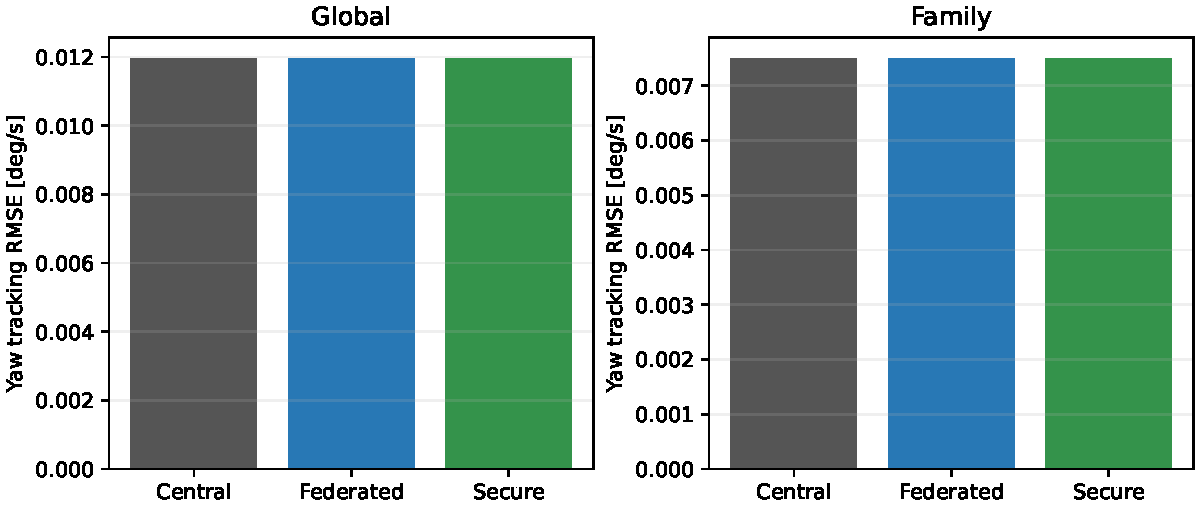
\includegraphics[width=0.82\linewidth]{../results/figures/experiment_8b_federated_equivalence.pdf}
\caption{Centralized, federated, and aggregate-only tracking results. The bars
overlap because discrepancies are many orders of magnitude smaller than the
performance scale.}
\label{fig:experiment8b}
\end{figure}

\Cref{tab:experiment8b,fig:experiment8b} confirms that the distributed
implementation changes neither the Global nor Family conclusion. Across all
federated and Secure fits, clients transmit 173,000 floating-point values and
receive 129,750 values. A typical oracle-Family fit requires roughly 35--37
objective evaluations: each participating client uploads four floats and receives
three per evaluation. These counts exclude identifiers, protocol metadata,
cryptographic keys, mask setup, retransmission, and secure-aggregation overhead.

\paragraph{Decision.}
The federated-equivalence gate passes. The project can now truthfully claim an
implemented distributed structured LPV estimator that keeps raw trajectories on
clients and reproduces centralized pooled optimization. The aggregate-only
emulator shows utility compatibility with secure summation, not formal privacy.
Experiment 8C may therefore introduce a specified client-level differential-
privacy mechanism and measure the resulting privacy--estimation--control frontier.
Family remains worse than Local as established in 7A--7C; 8B does not alter that
boundary result.

\paragraph{Reproducibility.}
The protocol is \path{code/config/experiment_8b.json}; the runner is
\path{code/experiments/experiment_8b_federated_equivalence.py}. The reusable
distributed optimizer is \path{code/src/federated_lpv/federated.py}. Compressed
per-seed outputs retain every fitted parameter, optimizer diagnostic, client
metric, and communication count. Aggregate equivalence tables and provenance
hashes are stored with the other experiment results.

\section{Experiment 8C: client-level privacy--control frontier}
\label{sec:experiment8c}

\paragraph{Question and threat model.}
Experiment 8C asks how formal client-level privacy affects structured LPV
estimation and downstream control. The protected unit is one vehicle's complete
local identification dataset. Replacement adjacency allows one participating
vehicle to be replaced by any other admissible vehicle. The adversary observes
only the released family aggregate; secure summation is assumed from 8B. The
mechanism does not hide the existence or size of a family, protect against
malicious clients, or include cryptographic overhead. Unlike secure aggregation
alone, differential privacy also limits information in the released aggregate.

\paragraph{One-shot bounded release.}
Every client first fits its local three-ratio model. Let $q_i=\log p_i$. Public
estimator bounds define a center $c$ and half-range vector $s$, giving
$z_i=(q_i-c)\oslash s\in[-1,1]^3$. The contribution is clipped to
$\lVert z_i\rVert_2\le C=\sqrt{3}$. For a family of $n=10$ clients, the
replacement sensitivity of the mean is
\begin{equation}
 \Delta_2=\frac{2C}{n}.
\end{equation}
The released normalized mean is
\begin{equation}
 \widetilde z=\frac1n\sum_{i=1}^n z_i+mathcal N(0,\sigma^2 I_3),
\end{equation}
where $\sigma$ is calibrated with the analytic Gaussian mechanism for the target
$(\epsilon,\delta)$ guarantee \cite{balle2018analytic}. Mapping $\widetilde z$
back into the public parameter box is post-processing. This one-shot release
avoids privacy composition across the iterative queries used in 8B, at the cost
of aggregating local estimates rather than the exact pooled output-error
objective.

\paragraph{Protocol.}
The privacy grid is $\epsilon\in\{0.5,1,2,4,8,\infty\}$ at
$\delta=10^{-5}$. Here $\epsilon=\infty$ is the non-private mean of the same
bounded client contributions. Ten independent privacy draws are evaluated on
each of ten fresh fleets, seeds 71--80, using the 7C single-speed local records.
Every released oracle-Family model is converted to the unchanged scheduled LQI
controller and tested on three nonlinear held-out scenarios. The descriptive
utility gate requires no more than 10\% mean tracking increase relative to the
non-private mean, full amplitude feasibility, and frozen spectral radius below
one. The relative threshold was fixed before execution.

\begin{table}[htbp]
\centering
\caption{Experiment 8C privacy--control frontier. Standard deviation and 95th
percentile use the 100 fleet--privacy-draw units at each finite $\epsilon$;
$\epsilon=\infty$ has ten fleet units.}
\label{tab:experiment8c}
\begin{tabular}{lrrrr}
\toprule
$\epsilon$ & Tracking mean & Tracking SD & Feasible fraction & Max. $\rho$\\
\midrule
0.5 & 1.38393 & 0.80278 & 0.89 & 5.3762\\
1 & 0.96284 & 0.75024 & 0.94 & 3.8755\\
2 & 0.45490 & 0.41700 & 0.99 & 3.4397\\
4 & 0.14038 & 0.09717 & 1.00 & 0.9896\\
8 & 0.06286 & 0.03668 & 1.00 & 0.9806\\
$\infty$ & 0.007432 & 0.000147 & 1.00 & 0.9691\\
\bottomrule
\end{tabular}
\end{table}

\begin{figure}[htbp]
\centering
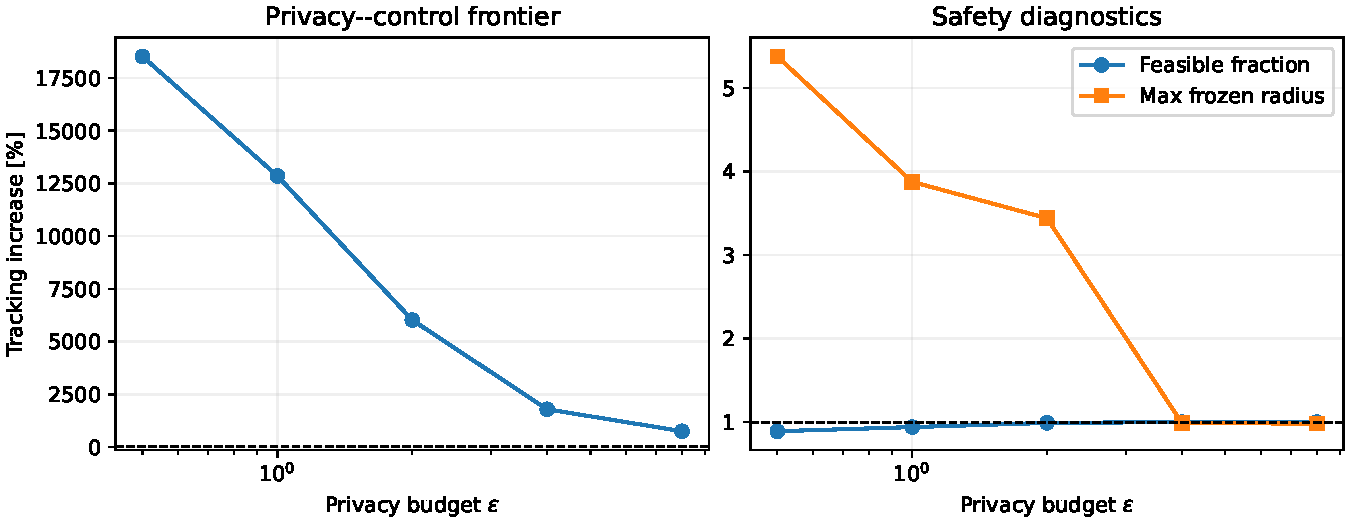
\includegraphics[width=0.86\linewidth]{../results/figures/experiment_8c_private_frontier.pdf}
\caption{Tracking degradation and safety diagnostics versus the client-level
privacy budget. Lower $\epsilon$ gives stronger privacy. The dashed line in the
left panel is the predeclared 10\% utility threshold; the dashed line in the
right panel marks frozen spectral radius one.}
\label{fig:experiment8c}
\end{figure}

\paragraph{Results and interpretation.}
All 300 local fits converge. The study evaluates 1,530 family releases and
45,900 client--scenario closed-loop cases. As \cref{tab:experiment8c,fig:experiment8c}
shows, no finite privacy level satisfies the 10\% gate. At $\epsilon=8$, mean
tracking error is 0.06286 deg/s, 746\% above the unusually small non-private
error of 0.007432 deg/s, although every run remains amplitude-feasible and the
largest frozen radius is 0.9806. At $\epsilon=4$, feasibility also remains
complete, but mean tracking reaches 0.14038 deg/s. For $\epsilon\le2$, at least
one privacy draw has frozen radius above one; feasibility rates are 0.99, 0.94,
and 0.89 for $\epsilon=2,1,0.5$, respectively. The low-$\epsilon$ results must
therefore not be summarized by mean tracking alone.

This failure is structural rather than an optimizer artifact. Replacement-level
sensitivity is $2\sqrt3/10$, so a group of ten provides limited privacy
amplification. Public parameter bounds are broad, and isotropic normalized noise
spends privacy budget on directions with unequal control relevance. Clipping the
released value to the parameter box prevents invalid parameters but cannot
recover the lost vehicle-specific information. Conversely, the large percentage
increases partly reflect an exceptionally accurate non-private baseline; the
absolute errors at $\epsilon=4$ and 8 may still be operationally small, but no
application-derived acceptance limit was available and none is introduced after
seeing the outcomes.

\paragraph{Decision.}
Naive one-shot isotropic client-level DP is not an acceptable final method for
ten-client families under the predeclared relative utility requirement. The
negative result nevertheless gives the FL extension a precise technical target.
The next experiment should test mechanisms that improve privacy utility without
weakening the definition: larger secure-aggregation cohorts, tighter defensible
public bounds, and control-sensitivity-aware anisotropic noise or projection.
Any such mechanism must retain the same $(\epsilon,\delta)$ adjacency statement
and be compared on fresh privacy draws. Record-level privacy or a larger
$\epsilon$ must not be substituted silently.

\paragraph{Reproducibility.}
The protocol is \path{code/config/experiment_8c.json}; the runner is
\path{code/experiments/experiment_8c_private_frontier.py}; analytic calibration
and transformations are in \path{code/src/federated_lpv/privacy.py}. Per-seed
compressed files retain local fits, every privacy draw, Gaussian scale, noise
norm, released parameter, and client-level closed-loop metrics.

\section{Experiment 8D: privacy-utility recovery}
\label{sec:experiment8d}

\paragraph{Question and fixed privacy statement.}
Experiment 8D tests whether the failed 8C utility gate can be recovered without
weakening its privacy definition. The protected unit remains one vehicle's
complete local dataset, adjacency remains replacement of one client, and
$\delta=10^{-5}$. The same analytic Gaussian calibration and one-shot family
mean release are used. Consequently, the only sensitivity reductions are a
smaller public log-parameter box and larger compatible secure-aggregation
cohorts; neither is a change from client-level to record-level privacy.

\paragraph{Protocol.}
The broad box from 8C is compared with the public benchmark-design box
$C_f/m\in[40,70]$, $C_r/m\in[35,75]$, and $m/I_z\in[0.45,0.8]$.
The latter is fixed from the declared admissible fleet design and is not fitted
to a participating client's records. Clipping remains part of the mechanism,
so the privacy guarantee also holds for an out-of-box contribution. No local
coordinate was clipped in this run. Tight-box cohorts contain 10, 30, or 100
clients per oracle family, with complementary speeds balanced over 10--30 m/s.
Five independent training fleets (seeds 81--85) are evaluated on separately
generated ten-client-per-family test fleets. Each finite
$\epsilon\in\{2,4,8\}$ uses ten privacy draws. The unchanged gate requires at
most 10\% mean tracking degradation relative to that mechanism's non-private
mean, full amplitude feasibility, and worst frozen spectral radius below one.

\begin{table}[htbp]
\centering
\caption{Experiment 8D privacy recovery. Tracking is mean yaw-rate RMSE in
deg/s. Increase is relative to the matching non-private cohort mean.}
\label{tab:experiment8d}
\begin{tabular}{llrrrr}
\toprule
Bounds/cohort & $\epsilon$ & Tracking & Increase & Feasible & Max. $\rho$\\
\midrule
Broad/10 & 2 & 0.37199 & 4632.12\% & 1.00 & 1.0457\\
Broad/10 & 4 & 0.14915 & 1797.37\% & 1.00 & 0.9913\\
Broad/10 & 8 & 0.06578 & 736.80\% & 1.00 & 0.9764\\
Tight/10 & 2 & 0.02162 & 174.99\% & 1.00 & 0.9732\\
Tight/10 & 4 & 0.01564 & 98.95\% & 1.00 & 0.9714\\
Tight/10 & 8 & 0.01100 & 39.91\% & 1.00 & 0.9703\\
Tight/30 & 2 & 0.01088 & 39.82\% & 1.00 & 0.9707\\
Tight/30 & 4 & 0.00908 & 16.60\% & 1.00 & 0.9698\\
Tight/30 & 8 & 0.00827 & 6.22\% & 1.00 & 0.9695\\
Tight/100 & 2 & 0.00825 & 6.05\% & 1.00 & 0.9692\\
Tight/100 & 4 & 0.00783 & 0.62\% & 1.00 & 0.9690\\
Tight/100 & 8 & 0.00779 & 0.09\% & 1.00 & 0.9688\\
\bottomrule
\end{tabular}
\end{table}

\begin{figure}[htbp]
\centering
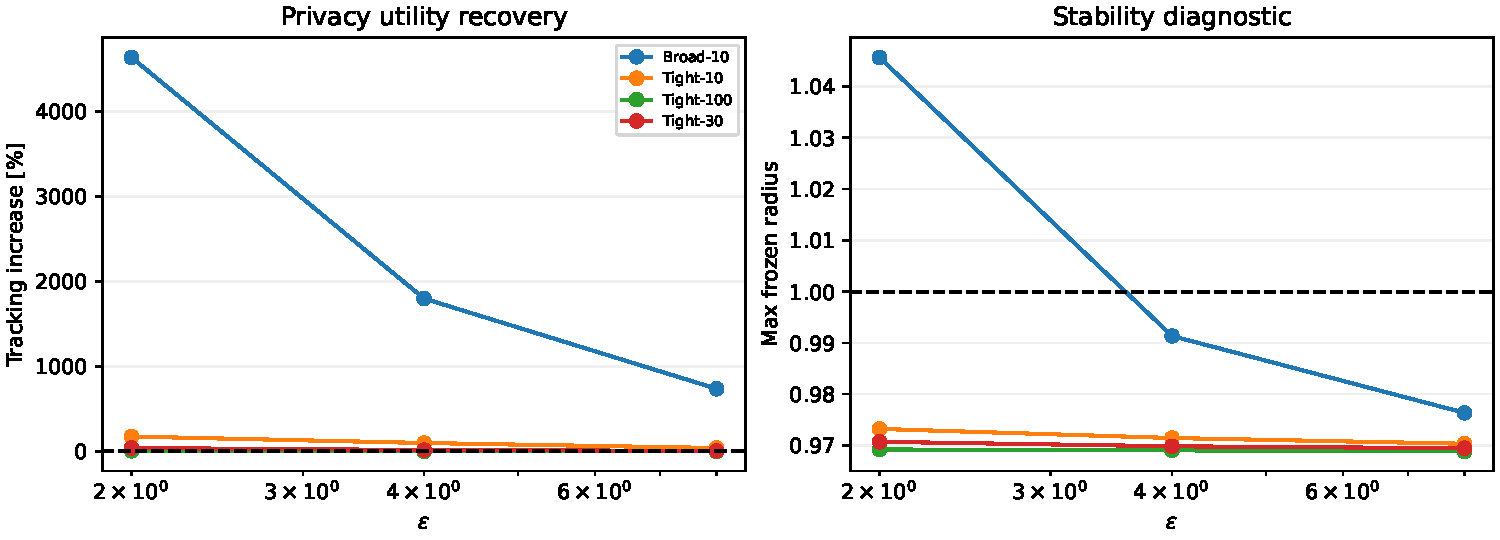
\includegraphics[width=0.9\linewidth]{../results/figures/experiment_8d_privacy_recovery.pdf}
\caption{Recovery from public bounds and cohort scaling. The left dashed line
marks the fixed 10\% tracking gate; the right dashed line marks frozen radius
one.}
\label{fig:experiment8d}
\end{figure}

\paragraph{Results.}
All 1,500 local fits converge. The run contains 1,860 family releases and
55,800 client--scenario evaluations. Tight/100 passes at every tested privacy
budget: degradation is 6.05\% at $\epsilon=2$, 0.62\% at $\epsilon=4$, and
0.09\% at $\epsilon=8$. Tight/30 first passes at $\epsilon=8$ with 6.22\%
degradation. Tight bounds alone greatly improve the ten-client result, but its
best finite cell still degrades tracking by 39.91\%. All cells are
amplitude-feasible, although Broad/10 at $\epsilon=2$ fails the frozen-radius
criterion. Thus the recovery gate passes because sensitivity scales as $1/n$
and the defensible box reduces the physical magnitude represented by a fixed
normalized perturbation.

\paragraph{Interpretation and limitations.}
The result supplies a concrete FL privacy benefit: compatible vehicles can
share a useful client-level-DP family model while retaining their trajectories
locally, provided the aggregation cohort is sufficiently large. It is not
evidence that ten-client fleets are adequate, that family labels can be exposed
safely, or that production secure aggregation has been implemented. Cohort
sizes 30 and 100 are simulated availability assumptions with full participation;
dropout, malicious clients, privacy accounting across repeated releases, and
learned private clustering remain open. The relative gate is also stringent
because non-private tracking is about 0.0078 deg/s; application-specific safety
limits should be established independently rather than inferred from this sweep.

\paragraph{Decision and reproducibility.}
Experiment 8D passes its recovery gate. The strongest tested passing point is
$\epsilon=2$ with 100 clients per family. This justifies proceeding to a
federated system study that treats cohort formation, partial participation, and
repeated releases explicitly. The frozen protocol is
\path{code/config/experiment_8d.json}; the runner is
\path{code/experiments/experiment_8d_privacy_recovery.py}; and aggregate results
are retained in \path{results/tables/experiment_8d_summary.csv} with compressed
per-seed fits, releases, and client metrics available from a full run.

\section{Experiment 8E: control-aware private aggregation}
\label{sec:experiment8e}

\paragraph{Question.}
Experiment 8E tests whether client-level privacy noise can be redistributed
toward directions that matter less for closed-loop control, while retaining the
replacement-adjacent $(\epsilon,\delta)$ guarantee from 8C--8D. The comparison
does not change the public parameter box, cohort, privacy budget, estimator, or
controller. It changes only the public geometry in which client contributions
are clipped and Gaussian noise is calibrated.

\paragraph{Mechanism and privacy argument.}
Let $z_i\in[-1,1]^3$ be client $i$'s bounded normalized log-parameter vector and
let $W_g=\operatorname{diag}(w_g)$ be a fixed positive diagonal matrix for
public compatibility class $g$. Define
\begin{equation}
 y_i=\Pi_{C_g}(W_gz_i),\qquad C_g=\lVert w_g\rVert_2,
\end{equation}
where $\Pi_{C_g}$ is Euclidean projection onto the radius-$C_g$ ball. This ball
contains the transformed public box, since
$\lVert W_gz\rVert_2\le\lVert w_g\rVert_2$ for every
$z\in[-1,1]^3$. The release is
\begin{equation}
 \widetilde z_g=W_g^{-1}\left(\frac{1}{n}\sum_{i=1}^{n}y_i+
 \xi\right),\qquad \xi\sim\mathcal N(0,\sigma_g^2I).
\end{equation}
Under replacement adjacency, the mean in transformed coordinates has
$\ell_2$ sensitivity $2C_g/n$. Calibrating $\sigma_g$ with the same analytic
Gaussian mechanism as 8C therefore gives $(\epsilon,\delta)$ client-level DP.
Multiplication by $W_g^{-1}$, conversion to physical parameters, parameter-box
projection, and controller synthesis are deterministic post-processing and do
not weaken the guarantee. Isotropic aggregation is the special case $W_g=I$.

The family-specific weights are public and frozen before private evaluation.
They are the normalized fourth roots of central finite-difference curvatures of
mean nonlinear yaw-tracking RMSE at the public family-center plants, using the
three declared design maneuvers and a step of 0.1 in normalized log coordinates.
For example, the nominal weights are $(1.636,1.820,0.336)$. Relative to isotropic
noise, this reduces normalized standard deviations in the two tire/mass ratios
to approximately 0.87 and 0.78, while increasing that of $m/I_z$ by a factor of
4.25. This allocation is justified only if the public curvature correctly
reflects downstream control relevance; Experiment 8E tests that premise.

\paragraph{Frozen protocol and gate.}
Ten fresh training fleets, seeds 86--95, contain 100 clients per family and use
the complementary single-speed recording protocol. Separate nonlinear test
fleets contain ten clients per family. Cohorts of 10, 30, and 100 are evaluated
at $\epsilon\in\{2,4,8,\infty\}$ and $\delta=10^{-5}$ over three held-out
maneuvers. Every finite cell uses ten privacy draws. Isotropic and control-aware
runs use common standard-normal draws for a paired comparison. Fleet means,
not individual clients or privacy draws, are the independent statistical units.
The gate, fixed before execution, requires at least one finite cell to achieve
all of: at least 15\% tracking improvement over isotropic DP, at most 10\%
degradation from the common non-private mean, complete amplitude feasibility,
and worst frozen radius below one.

\begin{table}[htbp]
\centering
\caption{Experiment 8E tracking results. ``Cost'' is degradation from the
common non-private mean; ``gain'' is improvement over isotropic DP.}
\label{tab:experiment8e}
\begin{tabular}{rrrrrr}
\toprule
$n$ & $\epsilon$ & Isotropic & Control-aware & Cost & Gain\\
\midrule
10 & 2 & 0.02169 & 0.01949 & 154.22\% & 10.16\%\\
10 & 4 & 0.01523 & 0.01349 & 76.03\% & 11.39\%\\
10 & 8 & 0.01094 & 0.01005 & 31.16\% & 8.10\%\\
30 & 2 & 0.01165 & 0.01063 & 39.52\% & 8.73\%\\
30 & 4 & 0.00886 & 0.00851 & 11.74\% & 3.97\%\\
30 & 8 & 0.00810 & 0.00796 & 4.48\% & 1.73\%\\
100 & 2 & 0.00812 & 0.00797 & 4.72\% & 1.86\%\\
100 & 4 & 0.00775 & 0.00771 & 1.30\% & 0.55\%\\
100 & 8 & 0.00767 & 0.00765 & 0.52\% & 0.19\%\\
\bottomrule
\end{tabular}
\end{table}

\begin{figure}[htbp]
\centering
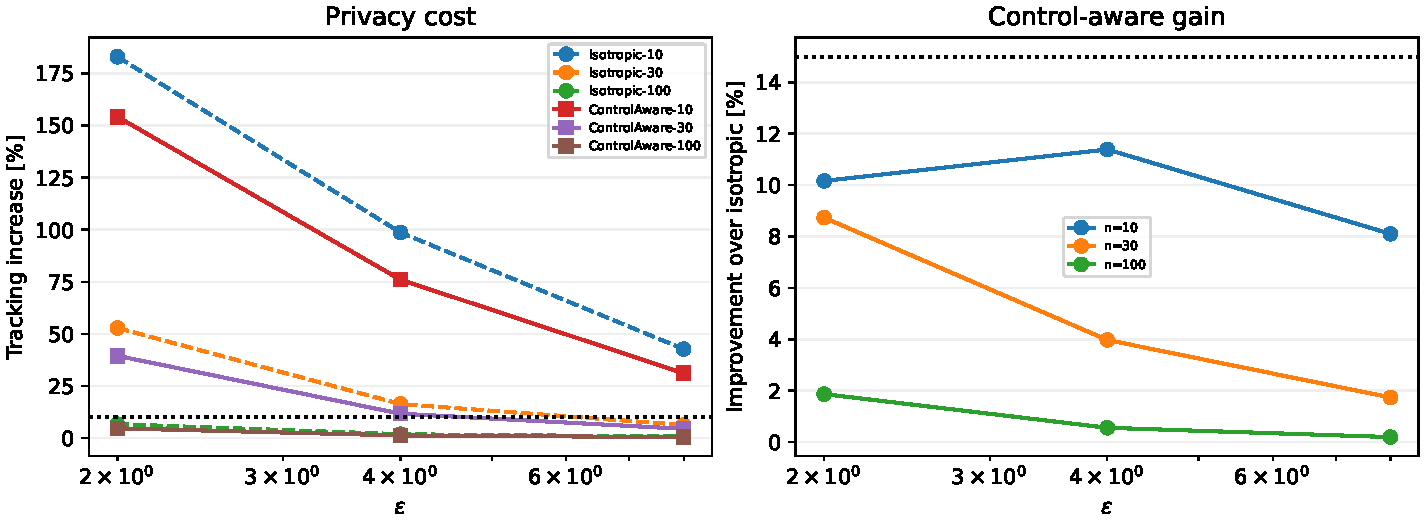
\includegraphics[width=0.9\linewidth]{../results/figures/experiment_8e_control_aware_privacy.pdf}
\caption{Privacy cost and improvement from public control-aware noise shaping.
The dashed thresholds are the frozen 10\% utility-cost and 15\% improvement
requirements.}
\label{fig:experiment8e}
\end{figure}

\paragraph{Results.}
All 3,000 local fits converge. The study retains 5,580 family releases and
167,400 client--scenario evaluations. No parameter coordinate or transformed
contribution is clipped, and every closed-loop evaluation is amplitude-feasible.
The control-aware method improves mean tracking in all nine finite cells and in
all ten independent fleets within every cell. A one-sided paired Wilcoxon test
on the ten fleet means gives $p=0.000977$ for every cell. The largest mean gain,
11.39\%, occurs for $n=10$, $\epsilon=4$; it does not reach the predeclared
15\% requirement. At the strategically important $n=30$, $\epsilon=4$ cell,
privacy cost falls from 16.36\% to 11.74\%, narrowly missing the 10\% utility
threshold. The $n=30$, $\epsilon=8$ and all $n=100$ cells satisfy the utility and
diagnostic conditions, but their improvements over isotropic DP are below 15\%.
Consequently, the joint control-aware gate fails.

\paragraph{Interpretation and decision.}
Public curvature shaping has a real and highly consistent directional effect,
but its practical magnitude is insufficient under the frozen criterion. The
benefit diminishes with cohort size because both mechanisms approach the same
non-private baseline. The result also shows why post-hoc threshold changes would
be misleading: $n=30$, $\epsilon=4$ is close to useful, yet it remains outside
the declared region. Experiment 8E must therefore be reported as a negative gate,
not as the final proposed-method validation.

The next step should not tune the diagonal weights on these private outcomes.
A defensible successor may derive a full public covariance from a stated
quadratic control-loss approximation and test it on new fleets, or retain the
simpler isotropic mechanism and focus the paper on the empirically established
cohort/privacy operating map. Partial participation and bound misspecification
remain necessary deployment tests under either choice.

\paragraph{Reproducibility.}
The frozen weights and protocol are in
\path{code/config/experiment_8e.json}; the shaped mechanism is implemented in
\path{code/src/federated_lpv/privacy.py}; and the runner is
\path{code/experiments/experiment_8e_control_aware_privacy.py}. Aggregate,
paired, and seed--draw summaries retain the complete reported evidence.

\section{Experiment 8F: deployment robustness of private federated LPV estimation}
\label{sec:experiment8f}

\paragraph{Question.}
Experiment 8F tests deployment effects omitted from Experiments 8C--8E:
partial participation, imperfect public clipping bounds, bounded outlying
contributions, and reduced tire--road friction. It replaces Experiment 8E's
arbitrary 15\% improvement criterion with an operational quantity: the minimum
cohort that keeps tracking degradation from its matching non-private aggregate
at or below 10\%.

\paragraph{Frozen protocol and gate.}
Ten fresh training fleets (seeds 96--105) contain 100 clients per family, with
separate nonlinear ten-client test fleets. Cohorts
$n\in\{10,20,30,50,100\}$ are selected by balanced, random, or deliberately
low-speed-biased policies. Isotropic and public control-aware mechanisms retain
replacement adjacency, $\delta=10^{-5}$, and
$\epsilon\in\{2,4,8,\infty\}$; common random draws enable paired comparisons.
A cell is viable when tracking cost is at most 10\%, every nonlinear run is
amplitude-feasible, and the worst frozen radius is below one.

Stage B fixes three $\epsilon=4$ points: $n=10$ (nonviable), $n=30$
(boundary), and $n=100$ (viable). It repeats them with the correct box, a box
narrowed by 10\%, a box shifted upward by 5\%, and 5\% or 10\% bounded outlier
contributions, at friction coefficients $\mu=0.9$ and $0.7$. The deployment
gate requires the viable point to pass all stresses. Outliers are adversarial
aggregation inputs projected by the mechanism, not new physical vehicle models.

\begin{table}[htbp]
\centering
\caption{Minimum viable cohort. All participation policies give the same minima.}
\label{tab:experiment8f-cohort}
\begin{tabular}{rrrr}
\toprule
$\epsilon$ & Isotropic & Control-aware & Cohort reduction\\
\midrule
2 & 100 & 100 & 0\%\\
4 & 50 & 50 & 0\%\\
8 & 30 & 20 & 33.3\%\\
\bottomrule
\end{tabular}
\end{table}

\begin{table}[htbp]
\centering
\caption{Tracking-cost ranges across both friction levels and all five stresses
at $\epsilon=4$.}
\label{tab:experiment8f-stress}
\begin{tabular}{lrrc}
\toprule
Point & Isotropic & Control-aware & All viable\\
\midrule
$n=10$ nonviable & 82.05--104.54\% & 63.28--81.74\% & no\\
$n=30$ boundary & 14.86--19.99\% & 10.67--14.33\% & no\\
$n=100$ viable & 0.18--2.02\% & $-0.04$--1.51\% & yes\\
\bottomrule
\end{tabular}
\end{table}

\begin{figure}[htbp]
\centering
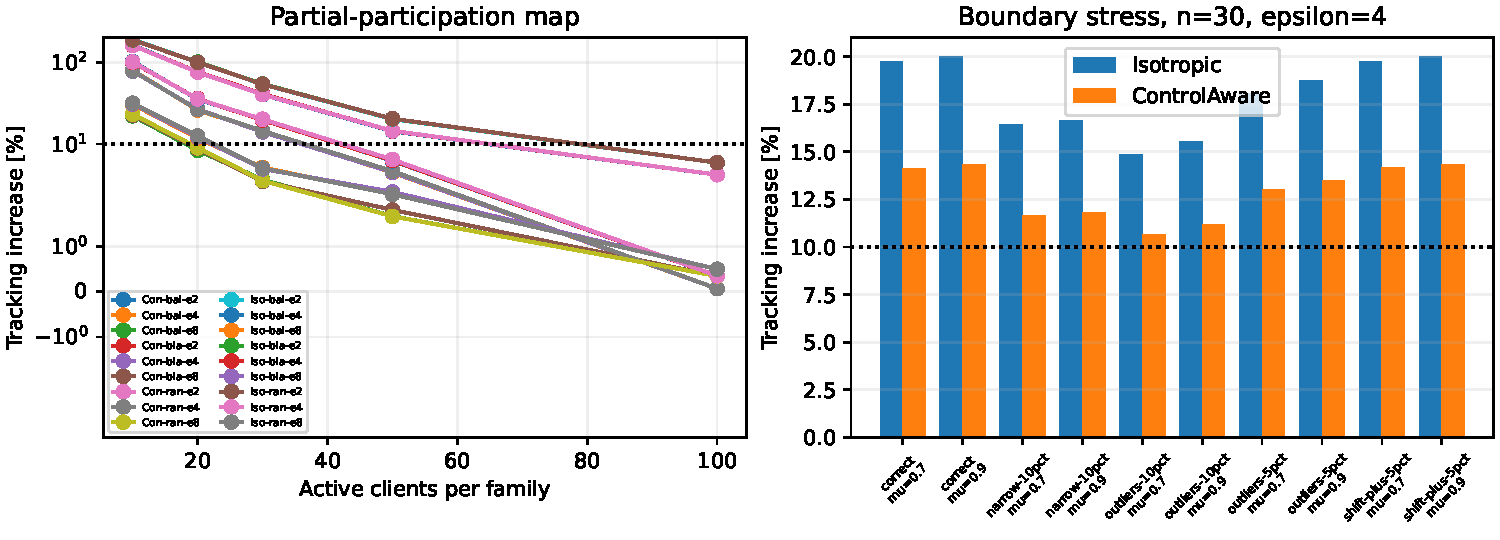
\includegraphics[width=0.93\linewidth]{../results/figures/experiment_8f_deployment_robustness.pdf}
\caption{Minimum viable cohort and deployment-stress results under the fixed
10\% tracking-cost boundary.}
\label{fig:experiment8f}
\end{figure}

\paragraph{Results.}
All 3,000 local fits converge. The experiment evaluates 25,200 private releases
and 756,000 nonlinear client--scenario combinations. All closed-loop runs are
amplitude-feasible and the largest frozen radius is below one. Minimum cohort is
insensitive to the tested participation policies. For control-aware privacy it
is 100, 50, and 20 at $\epsilon=2,4,8$; isotropic privacy requires 100, 50, and
30. Hence shaping reduces the required cohort by one third at $\epsilon=8$.

At $n=100,\epsilon=4$, both mechanisms pass every Stage B stress. Their largest
tracking costs are 2.02\% (isotropic) and 1.51\% (control-aware), including at
$\mu=0.7$. Neither mechanism makes the $n=30$ or $n=10$ point viable under all
stresses, preserving the boundary of the supported region. In total 16,224
released coordinates are projected to a public box, so clipping is active.

\paragraph{Interpretation and limitations.}
Experiment 8F passes its deployment gate. The supported claim is an empirical
cohort--privacy operating region that remains valid under the stated bounded
perturbations. Control-aware shaping reduces cohort size in one regime; it is
not universally superior. The participation finding is benchmark-specific,
the outlier test is not Byzantine security, and privacy covers one release
rather than repeated-round composition.

\paragraph{Reproducibility.}
The design is in \path{code/config/experiment_8f.json}; the runner is
\path{code/experiments/experiment_8f_deployment_robustness.py}. Friction is
propagated by \path{code/experiments/experiment_6b_acceleration_validation.py}.
Aggregate and seed-level evidence is retained under \path{results/tables}.

\section{Experiment 8G: blind end-to-end confirmation}
\label{sec:experiment8g}

\paragraph{Question and frozen predictions.}
Experiment 8G prevents the operating map in Experiment 8F from serving as both
discovery and confirmation. On ten new fleet seeds (106--115), it tests two
points chosen before execution. The primary prediction is that control-aware DP
is viable and isotropic DP is not at $n=20,\epsilon=8$. The secondary prediction
is that both are viable at $n=50,\epsilon=4$. Viability retains the 10\%
tracking-cost limit, full nonlinear amplitude feasibility, and frozen radius
below one. The primary gate additionally requires control-aware improvement in
all ten fleet seeds.

Each test fleet is separate from its training fleet. The comparison includes a
three-second Local fit for every test vehicle, the non-private compatible-family
aggregate, isotropic client-level DP, and control-aware client-level DP. Ten
privacy draws use common random numbers. Local superiority is neither required
nor claimed; its inclusion makes the collaboration tradeoff explicit.

\begin{table}[htbp]
\centering
\caption{Blind Experiment 8G results. Tracking cost is relative to the matching
non-private family aggregate.}
\label{tab:experiment8g}
\begin{tabular}{lrrr}
\toprule
Method & $n=20,\epsilon=8$ & $n=50,\epsilon=4$ & Feasible\\
\midrule
Local & $-11.90$\% & $-11.32$\% & yes\\
Family non-private & 0.00\% & 0.00\% & yes\\
Isotropic DP & 14.40\% & 5.08\% & yes\\
Control-aware DP & 10.43\% & 3.48\% & yes\\
\bottomrule
\end{tabular}
\end{table}

\begin{figure}[htbp]
\centering
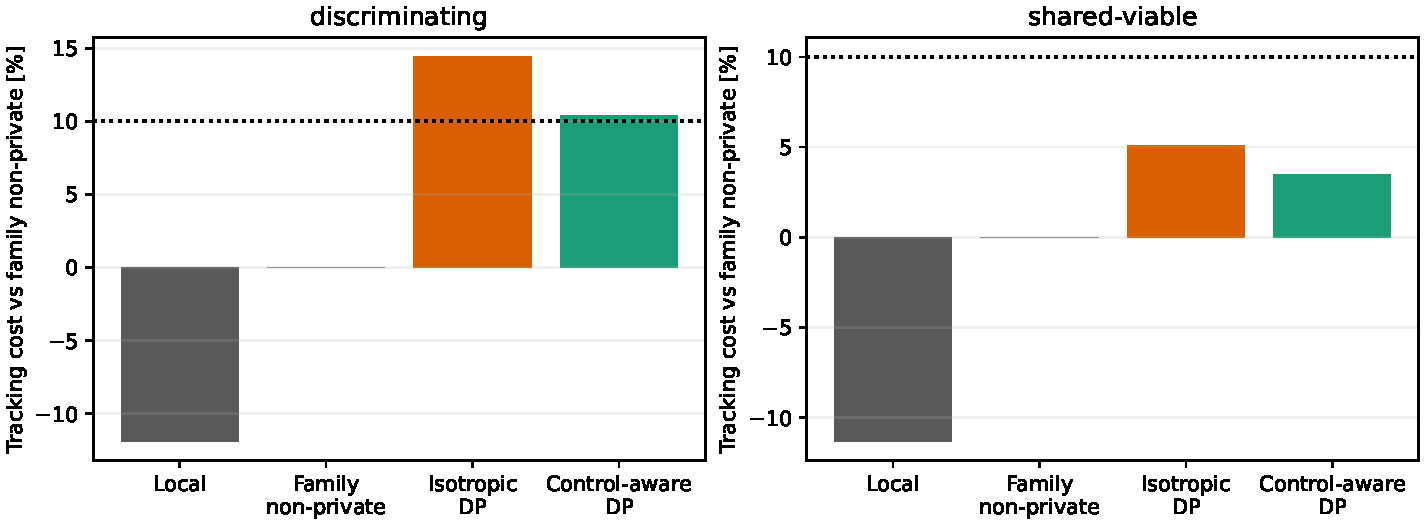
\includegraphics[width=0.9\linewidth]{../results/figures/experiment_8g_blind_confirmation.pdf}
\caption{Blind comparison at the two frozen deployment points. The dotted line
is the unchanged 10\% tracking-cost boundary.}
\label{fig:experiment8g}
\end{figure}

\paragraph{Results.}
All 1,800 local fits converge. The run contains 1,200 private family releases
and 39,600 nonlinear client--scenario evaluations. All methods are
amplitude-feasible and have worst frozen radius below one. At the primary point,
control-aware DP improves on isotropic DP in every fleet seed, with a 3.47\%
mean gain and one-sided paired Wilcoxon $p=0.000977$. Nevertheless, its 10.43\%
cost narrowly exceeds the frozen limit; isotropic DP costs 14.40\%. The primary
confirmation gate therefore fails. At the secondary point, both mechanisms
confirm as viable: control-aware DP costs 3.48\% and isotropic DP 5.08\%.

Local identification has the best absolute tracking and lower mean parameter
error. Its tracking is 11.90\% and 11.32\% better than the respective
non-private family aggregates. This repeats the earlier boundary finding that
federation does not improve a highly efficient Local estimator in this
benchmark; the supported benefits are privacy-preserving shared calibration and
model consolidation.

\paragraph{Decision.}
Experiment 8G is a negative primary gate and a positive secondary confirmation.
The manuscript must not claim that 20 clients suffice at $\epsilon=8$ under a
strict 10\% criterion. Its headline confirmed point is instead
$n=50,\epsilon=4$, while the 20-client outcome defines a close but unsupported
boundary. The all-seed directional improvement supports control-aware shaping,
but does not override the failed absolute-utility criterion. No post-hoc
threshold or weight adjustment is warranted.

\paragraph{Reproducibility.}
The frozen protocol is in \path{code/config/experiment_8g.json}; the runner is
\path{code/experiments/experiment_8g_blind_confirmation.py}. Aggregate,
seed--draw, paired, and conclusion files are stored under \path{results/tables}.

\section{Experiment 9A: learned compatibility groups}
\label{sec:experiment9a}

\paragraph{Question.}
Experiment 9A asks whether useful sharing groups and their number can be learned
from compact local LPV estimates rather than supplied as oracle family labels.
It is deliberately non-private: privacy-aware cluster sizing and protection of
cluster discovery are deferred until useful grouping itself passes a hard gate.
Training vehicles determine the partition and cluster models; separate unseen
vehicles are assigned by their local three-ratio estimate. Simulator family
labels enter only the oracle baseline and post-hoc adjusted Rand index (ARI).

\paragraph{Methods and frozen selection.}
Ten fresh fleets (seeds 116--125) contain 60 training and ten unseen test
vehicles per simulated family. All clients receive three one-second,
single-speed records. The methods are Local (30 test-vehicle models), Global
(one model), Oracle family (three models), ordinary $K$-means with fixed $K=3$,
and two learned-$K$ variants. Parameter clustering operates on publicly bounded
normalized log-ratios. Control clustering multiplies all clients by one public,
label-independent diagonal metric derived at the nominal public plant; it does
not use family-specific weights.

Learned $K$ maximizes training silhouette over $K\in\{2,\ldots,8\}$, subject to
at least ten training clients per cluster. If no candidate exceeds 0.25, the
method selects $K=1$. Unseen assignments use the nearest training centroid.
The hard gate requires learned-$K$ control clustering to track no worse than the
oracle-family model, remain amplitude-feasible with frozen radius below one,
and deploy fewer models than Local.

\begin{table}[htbp]
\centering
\caption{Experiment 9A unseen-client results.}
\label{tab:experiment9a-results}
\begin{tabular}{lrrrr}
\toprule
Method & Tracking & Models & Parameter error & Worst client\\
\midrule
Local & 0.006692 & 30.0 & 0.0230 & 0.007397\\
Global & 0.011700 & 1.0 & 0.1299 & 0.018969\\
Oracle family & 0.007556 & 3.0 & 0.0469 & 0.010510\\
Fixed $K=3$ & 0.007554 & 3.0 & 0.0469 & 0.010500\\
Learned-$K$ parameter & 0.007554 & 3.0 & 0.0469 & 0.010500\\
Learned-$K$ control & 0.007757 & 2.9 & 0.0497 & 0.011256\\
\bottomrule
\end{tabular}
\end{table}

\begin{table}[htbp]
\centering
\caption{Learned partition diagnostics averaged over ten fleets.}
\label{tab:experiment9a-clusters}
\begin{tabular}{lrrrr}
\toprule
Method & $K$ range & Train ARI & Test ARI & Silhouette\\
\midrule
Fixed $K=3$ & 3--3 & 0.987 & 1.000 & 0.537\\
Learned-$K$ parameter & 3--3 & 0.987 & 1.000 & 0.537\\
Learned-$K$ control & 2--3 & 0.915 & 0.951 & 0.572\\
\bottomrule
\end{tabular}
\end{table}

\begin{figure}[htbp]
\centering
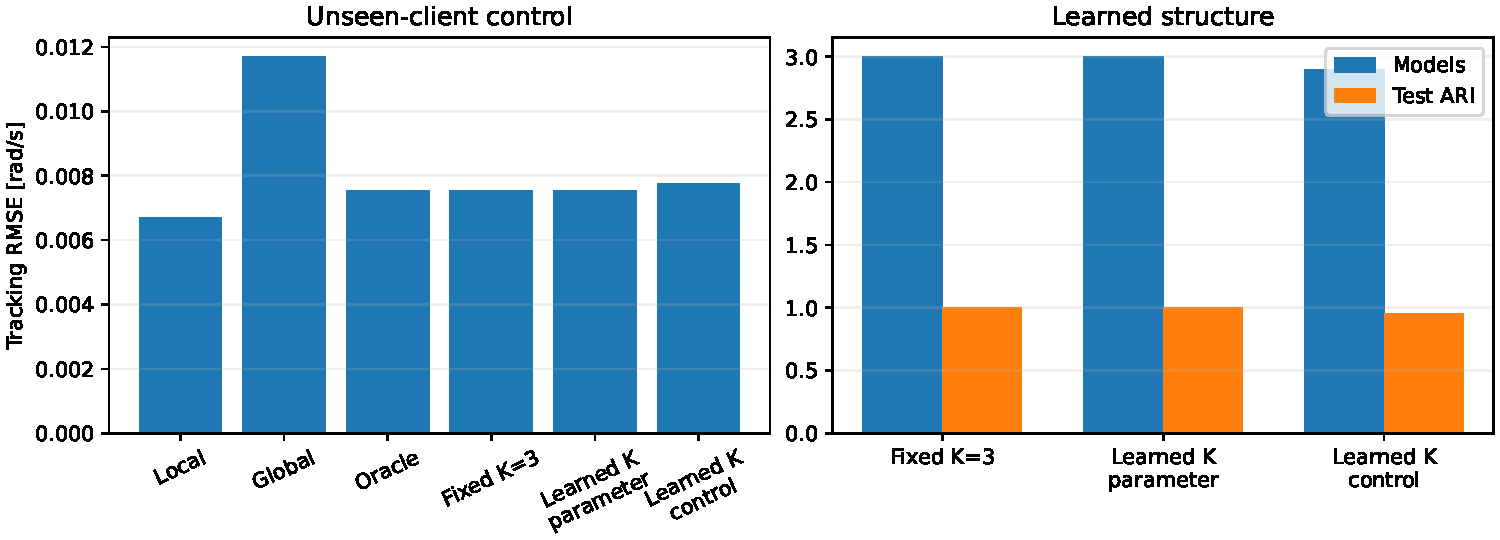
\includegraphics[width=0.93\linewidth]{../results/figures/experiment_9a_learned_groups.pdf}
\caption{Unseen-client tracking and learned grouping structure in Experiment
9A. ARI is diagnostic only and is not used for model selection.}
\label{fig:experiment9a}
\end{figure}

\paragraph{Results.}
All 2,100 local fits converge and all 5,400 nonlinear evaluations are
amplitude-feasible with frozen radius below one. Learned-$K$ parameter
clustering selects three groups in every fleet. Its training ARI is 0.987, while
nearest-centroid assignment reaches test ARI 1.0 on all unseen vehicles. Its
tracking RMSE, 0.007554 rad/s, is effectively equal to and slightly below the
oracle-family value of 0.007556 rad/s. It therefore removes the label assumption
for this discrete-family benchmark while retaining three deployed controllers
instead of 30 Local controllers. Local remains 11.4\% better in tracking, and
Global is 54.8\% worse than oracle family.

The learned-$K$ control variant fails the hard gate. It chooses $K=2$ on seed
124, merges incompatible groups (test ARI 0.506), and increases that fleet's
tracking error by 25.5\% relative to oracle. Across all fleets it is 2.66\%
worse than oracle. Its higher silhouette shows why geometric compactness alone
is insufficient: the public curvature used to allocate DP noise suppresses a
parameter direction that remains important for deciding which clients should
share a controller.

\paragraph{Decision and limitations.}
Experiment 9A supports label-free parameter-space compatibility discovery, but
rejects direct reuse of the control-aware privacy geometry for clustering. The
positive result is presently limited by the simulator's clearly discrete three-
family construction. Before it becomes a strong paper contribution, Experiment
9B must test shorter/noisier identification, unbalanced populations, and
continuous heterogeneity. Moreover, the server currently observes individual
local estimates; this is trusted-server clustering, not end-to-end private
group discovery. Privacy-aware clustering should proceed only if 9B confirms
stable useful partitions beyond this favorable discrete setting.

\paragraph{Reproducibility.}
The frozen protocol is in \path{code/config/experiment_9a.json}; implementation
is in \path{code/experiments/experiment_9a_learned_groups.py}. Seed summaries,
candidate scores, selected-cluster diagnostics, and conclusions are retained
under \path{results/tables}.


\bibliographystyle{plain}
\bibliography{references}
\end{document}
